\documentclass[a4paper,12pt]{article}
\usepackage[left=2cm,right=1cm,top=1cm,bottom=1.5cm]{geometry}
\usepackage[utf8]{inputenc}
\usepackage[english,russian]{babel}
\usepackage{graphicx}
\usepackage{amsmath}
\usepackage{amssymb}
\usepackage{cite}
\usepackage{indentfirst}
\usepackage{multicol}
\usepackage{cmap}
\usepackage{hyperref}
\usepackage{esint}
\usepackage{listings}
%\usepackage{minted}
\usepackage{xcolor}
%\usepackage{inconsolata}
%\renewcommand*\familydefault{\ttdefault} %% Only if the base font of the document is to be typewriter style
%\usepackage[T1]{fontenc}
\hypersetup{
	colorlinks=true,
	linkcolor=black,
	filecolor=black,  
	urlcolor=blue,
	pdftitle={Overleaf Example},
	pdfpagemode=FullScreen,
}

\sloppy

\usepackage{geometry}
\geometry{top=2cm}
\geometry{bottom=2cm}
\geometry{left=2.5cm}
\geometry{right=2.5cm}

\renewcommand{\baselinestretch}{1.5}

	\newcommand{\ds}{\displaystyle}
	\renewcommand{\phi}{\varphi}
	\newcommand{\sgn}{\, \text{sgn} \,}
	\renewcommand{\a}{\alpha}
	\renewcommand{\b}{\beta}
	\renewcommand{\l}{\lambda}
	\renewcommand{\d}{\partial}
	\renewcommand{\^}[2]{#1^{\, #2} \kern -1pt}
	\newcommand{\veco}{\kern -1pt \vec{\kern 1pt 0}}
	\newcommand{\1}{\kern 1pt}
	\newcommand{\0}{\kern -1pt}
	\renewcommand{\Phi}{\varPhi}
	

\begin{document}
	\renewcommand{\contentsname}{\Large Содержание}
	\renewcommand{\bibname}{\normalfont\Large\bfseries Список литературы}
	
	\begin{titlepage}
		\begin{center}
			\tiny{МИНИСТЕРСТВО НАУКИ И ВЫСШЕГО ОБРАЗОВАНИЯ РОССИЙСКОЙ ФЕДЕРАЦИИ\\
			ФЕДЕРАЛЬНОЕ ГОСУДАРСТВЕННОЕ АВТОНОМНОЕ ОБРАЗОВАТЕЛЬНОЕ УЧРЕЖДЕНИЕ\\
			ВЫСШЕГО ОБРАЗОВАНИЯ}\\
			\normalsize{\textbf{Национальный исследовательский ядерный университет «МИФИ»}}\\*
			\hrulefill
		\end{center}
		\vspace{0.5cm}
		
		\begin{center}
			\large{\textbf{Институт}\\
			\textbf{интеллектуальных кибернетических систем}}
		\end{center}
		\vspace{0.5cm}
		
		\begin{center}
			\large{\textbf{Кафедра кибернетики (№ 22)}}
		\end{center}
		
		\vspace{0.5cm}
		
		\begin{center}
			\large{\textbf{Отчёт о работе по курсу}\\
			\textbf{«Базы данных (теоретические основы баз данных)»}}
		\end{center}
		
		\begin{center}
			\large \underline{Вариант «Онлайн кассы для сети кинотеатров»}
		\end{center}
		\vspace{1.0cm}
		
		\begin{flushright}
			\begin{tabular}{|l|c|}
				\hline
				Выполнил      & Рокин О.Д.      \\ \hline
				Группа        & Б21-215         \\ \hline
				Вариант 	  & \begin{tabular}[c]{@{}c@{}}Онлайн кассы для\\ сети кинотеатров\end{tabular} \\ \hline
				Преподаватель & Миркасымов Р.Б. \\ \hline
				Проверяющий   &                 \\ \hline
				Оценка        &                 \\ \hline
			\end{tabular}
		\end{flushright}
		
		
		\vspace{15em}
		
		\begin{center}
			\textbf{Москва 2023}
		\end{center}
	\end{titlepage}
	
	\newpage 
	\tableofcontents
	\setcounter{page}{2}
	
	\newpage
	
	\section{Формулировка задания}
	
	\newpage
	
	\section{Концептуальная модель базы данных}
	
	После проведения анализа предметной области была спроектирована следующая концептуальная модель:
	
	\begin{figure}[h]
		\hspace{-1.75cm}
		\includegraphics[scale=0.094,page=1]{Концептуальная модель.pdf}
		\caption{Концептуальная модель базы данных}
	\end{figure}
	
	\newpage
	
	\subsection{Конкретизация предметной области}
	
	\newpage
	
	\subsection{Описание предметной области}
	
	Таким образом, были выделены следующие сущности:
	
	\begin{itemize}
		\setlength\itemsep{0.05cm}
		
		\item Фильмы
		
		\item Изображения
		
		\item Жанры
		
		\item Члены съёмочной группы
		
		\item Номинации
		
		\item Награды
		
		\item Сеансы
		
		\item Билеты
		
		\item Заказы
		
		\item Оплата
		
		\item Пользователи
		
		\item Залы
		
		\item Сиденья
		
		\item Кинотеатры
		
		\item Сотрудники
		
		\item Должности в кинотеатре
	\end{itemize}
	
	\newpage
	
	\subsection{Описание атрибутов}
	
	В процессе анализа были выделены следующие атрибуты, название и описание которых приведены в таблице ниже.
	
	\begin{center}
		\begin{tabular}{|p{4cm}|p{4cm}|p{7cm}|}
			\hline
			\textbf{Имя сущности}	& \textbf{Имя атрибута} 	& \textbf{Расшифровка}	\\ \hline
			Фильмы	& Название	& Название фильма (необязательно уникальное)	\\ \hline
			Фильмы	& Дата выхода	& Дата выхода фильма	\\ \hline
			Фильмы	& Длительность	& Длительность фильма	\\ \hline
			Фильмы	& Возрастное ограничение	& Возрастное ограничение фильма (PG-13, R и т.п.)	\\ \hline
			Фильмы	& Описание	& Описание к фильму	\\ \hline
			Фильмы	& Рейтинг	& Рейтинг/оценка фильма	\\ \hline
			Фильмы	& Ссылка на Кинопоиск	& Ссылка на страницу фильма на сайте kinopoisk.ru	\\ \hline
			Изображения	& Ссылка	& Ссылка на изображение к фильму	\\ \hline
			Изображения	& Постер?	& Отвечает, является ли изображение постером к фильму, или просто кадром/скриншотом	\\ \hline
			Жанры	& Название	& Название жанра фильма	\\ \hline
			Члены съёмочной группы	& Имя	& Полное имя члена съёмочной группы (необязательно уникальное)	\\ \hline
			Члены съёмочной группы	& Дата рождения	& Дата рождения члена съёмочной группы	\\ \hline
			Члены съёмочной группы	& Место рождения	& Место рождения члена съёмочной группы	\\ \hline
			Члены съёмочной группы	& Рост	& Рост члена съёмочной группы (важно для актёров)	\\ \hline
			Номинации	& Название	& Название номинации (за лучшую мужскую роль, за лучшую роль второго плана и т.п.)	\\ \hline
		\end{tabular}
	\end{center}

	\begin{center}
		\begin{tabular}{|p{4cm}|p{4cm}|p{7cm}|}
			\hline
			Номинации	& Статус	& Отвечает, оказался ли номинант победителем	\\ \hline
			Номинации	& Год	& Год выдвижения номинации	\\ \hline
			Награды	& Название	& Название награды (Оскар, Золотой глобус и т.п.)	\\ \hline
			Сеансы	& Время начала	& Время начала сеанса	\\ \hline
			Сеансы	& Время окончания	& Время окончания сеанса	\\ \hline
			Билеты	& Цена	& Цена за билет (может различаться даже в пределах одного зала)	\\ \hline
			Заказы	& Забронирован?	& Отвечает, забронирован ли заказ, или его только начали оформлять	\\ \hline
			Заказы	& Полная стоимость	& Полная стоимость заказа (вычисляется как сумма цен за билеты)	\\ \hline
			Оплата	& Способ оплаты	& Способ оплаты (оплата наличными на месте, оплата банковской картой онлайн и т.п.)	\\ \hline
			Оплата	& Время оплаты	& Время, когда была произведена оплата	\\ \hline
			Пользователи	& Имя	& Полное имя пользователя (необязательно уникальное)	\\ \hline
			Пользователи	& Дата рождения	& Дата рождения пользователя	\\ \hline
			Пользователи	& Логин	& Логин пользователя	\\ \hline
			Пользователи	& Пароль	& Пароль пользователя	\\ \hline
			Пользователи	& Телефон	& Номер телефона пользователя	\\ \hline
			Пользователи	& Почта	& Электронная почта пользователя	\\ \hline
			Пользователи	& Аватар	& Ссылка на изображение, являющееся аватаром пользователя	\\ \hline
			Залы	& Название/Номер	& Название/Номер зала	\\ \hline
			Залы	& Тип	& Тип зала (стандартный, VIP и т.п.)	\\ \hline
			Сиденья	& Ряд	& Ряд сиденья	\\ \hline
			Сиденья	& Место	& Место сиденья	\\ \hline
			Кинотеатры	& Название	& Название кинотеатра	\\ \hline
			Кинотеатры	& Адрес	& Адрес кинотеатра	\\ \hline
		\end{tabular}
	\end{center}

	\begin{center}
		\begin{tabular}{|p{4cm}|p{4cm}|p{7cm}|}
			\hline
			Кинотеатры	& Телефон	& Официальный номер телефона кинотеатра	\\ \hline
			Сотрудники	& Имя	& Полное имя сотрудника (необязательно уникальное)	\\ \hline
			Сотрудники	& Дата рождения	& Дата рождения сотрудника	\\ \hline
			Сотрудники	& Логин	& Логин сотрудника	\\ \hline
			Сотрудники	& Пароль	& Пароль сотрудника	\\ \hline
			Сотрудники	& Телефон	& Номер телефона сотрудника	\\ \hline
			Сотрудники	& Почта	& Электронная почта сотрудника	\\ \hline
			Должности в кинотеатре	& Название	& Название должности сотрудника в кинотеатре	\\ \hline
		\end{tabular}
	\end{center}
	
	\newpage
	
	\section{Логическое проектирование}
	
	Следующим шагом на основе КМПО была разработана логическая модель базы данных, представленная ниже:
	
	\begin{figure}[h]
		\hspace{-1.75cm}
		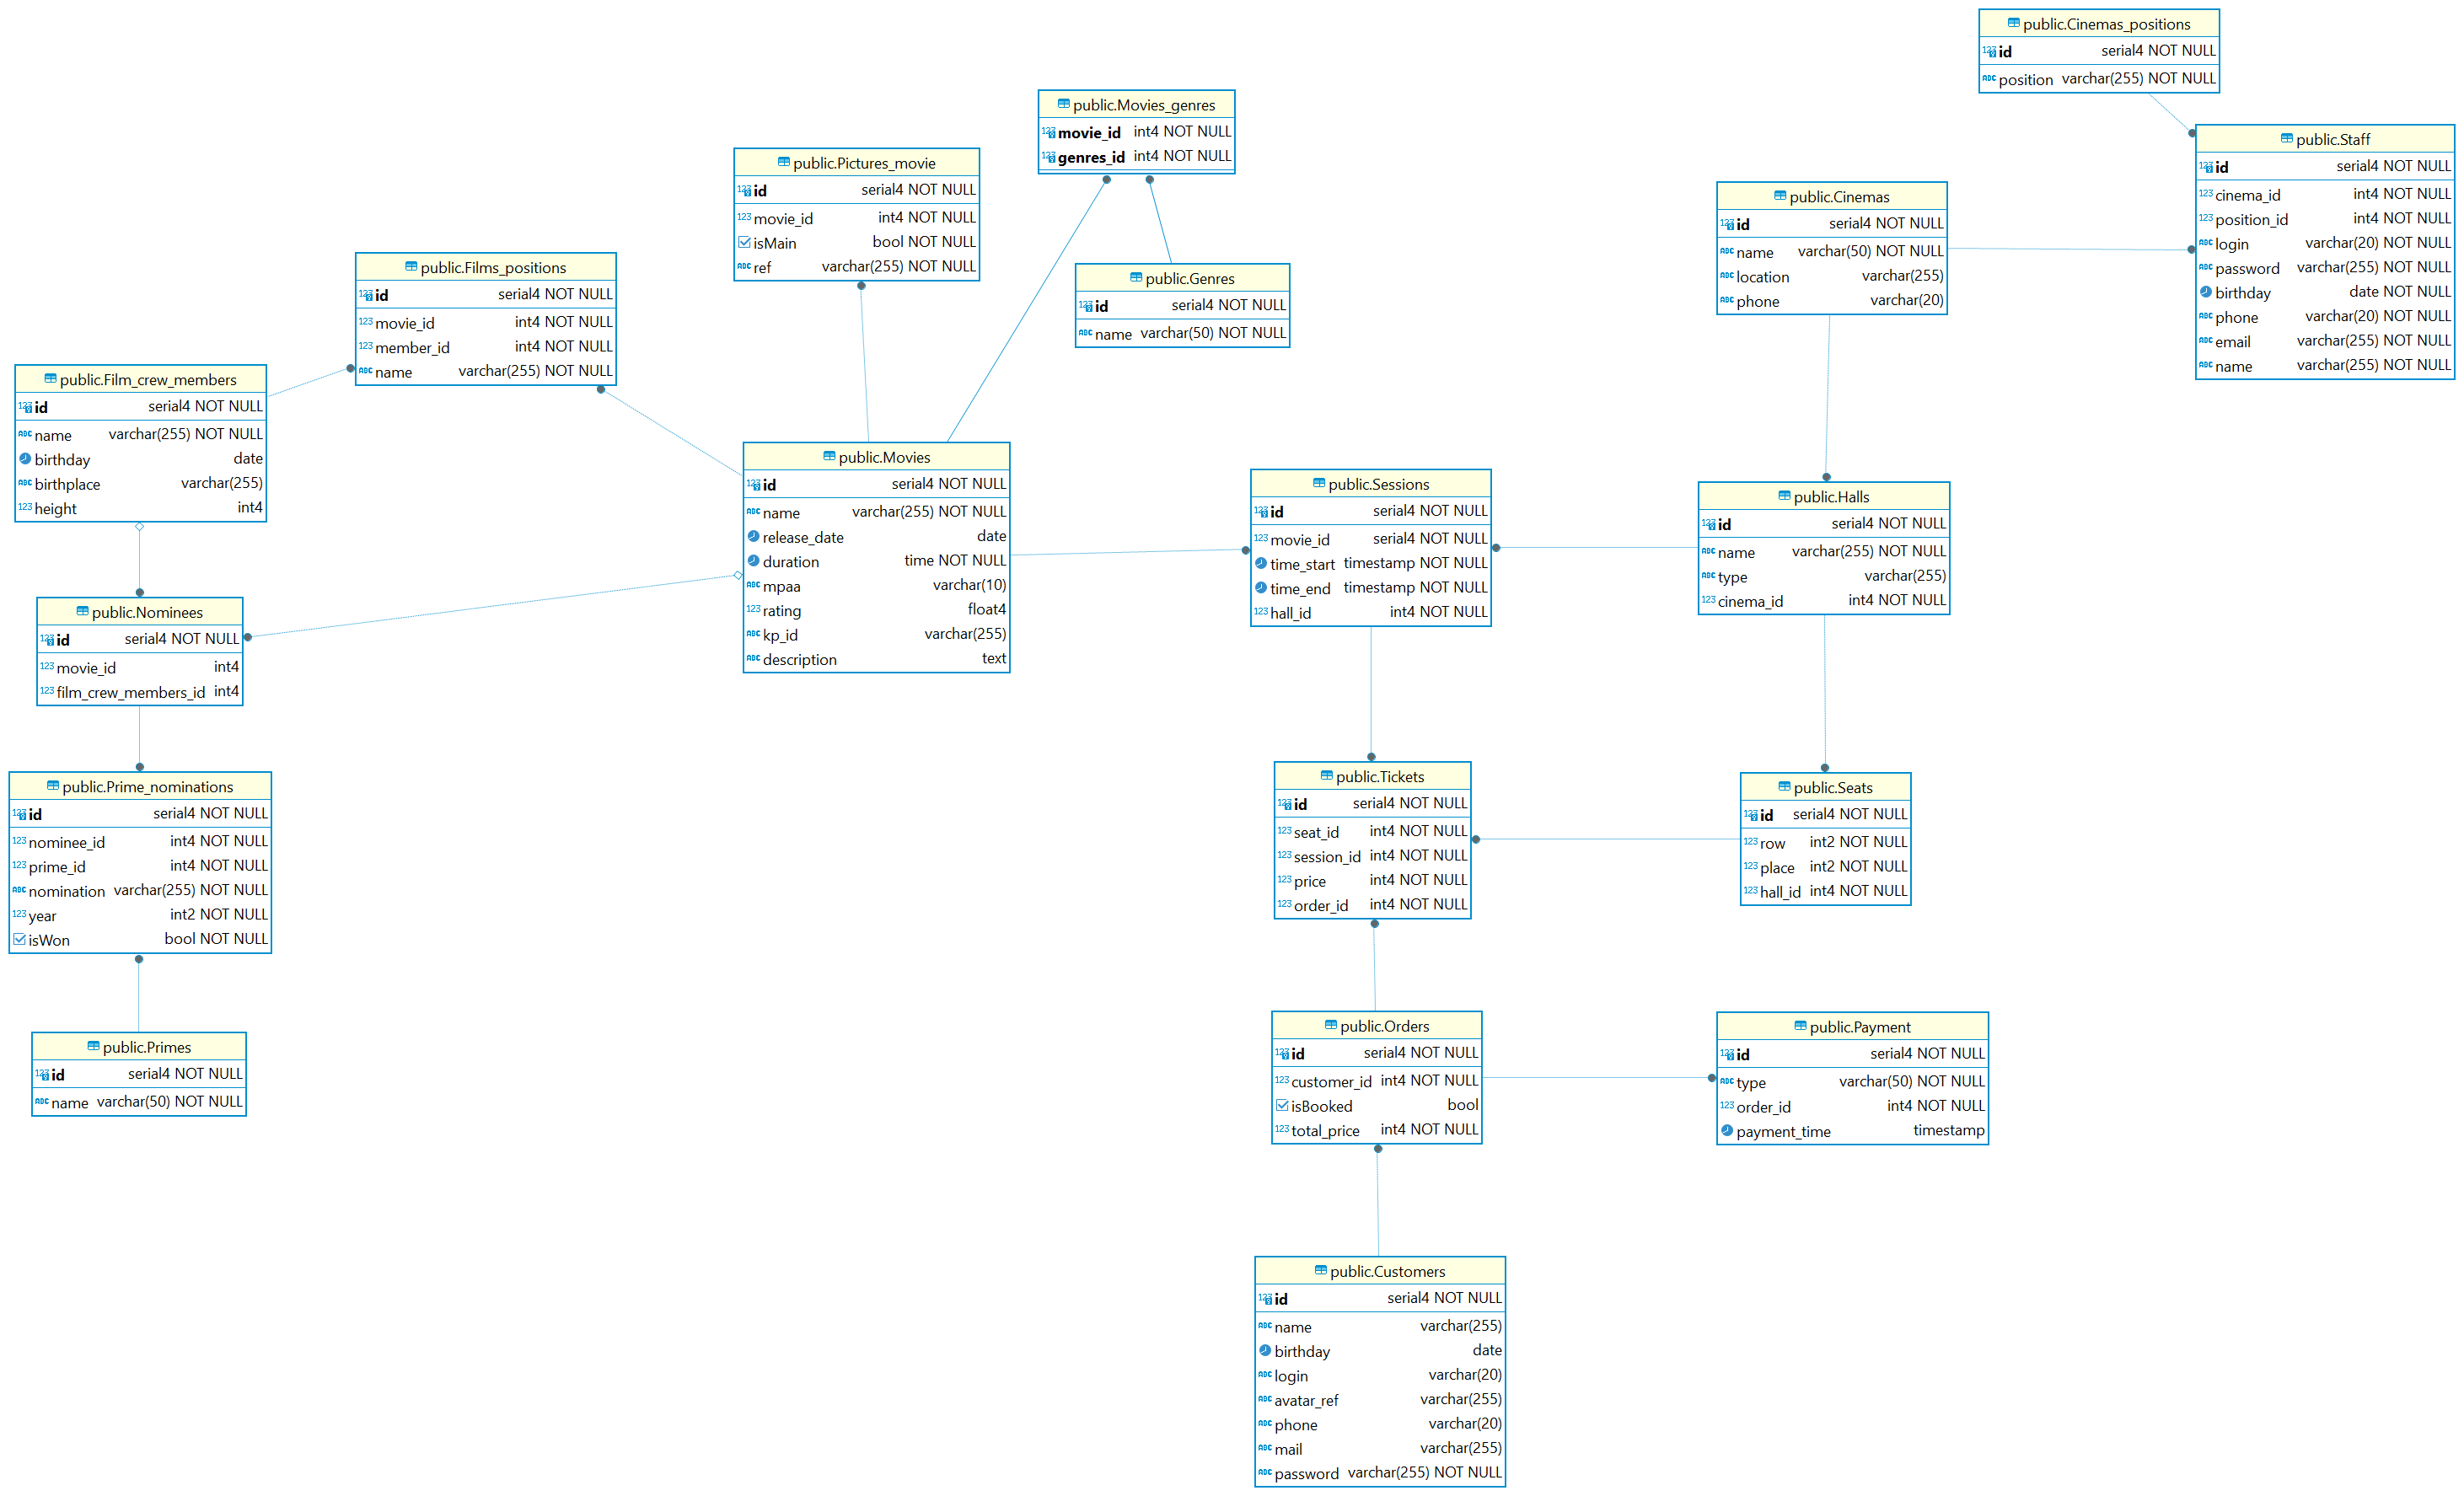
\includegraphics[scale=0.19,page=1]{Логическая модель.png}
		\caption{Логическая модель базы данных}
	\end{figure}
	
	\newpage
	
	\section{Физическое проектирование}
	
	В качестве СУБД для реализации разработанной базы данных была выбрана PostgreSQL. В связи с проведённым анализом предметной области и была проработана следующая физическая схема базы данных. Она представлена на следующем рисунке:
	
	\begin{figure}[h]
		\hspace{-1.75cm}
		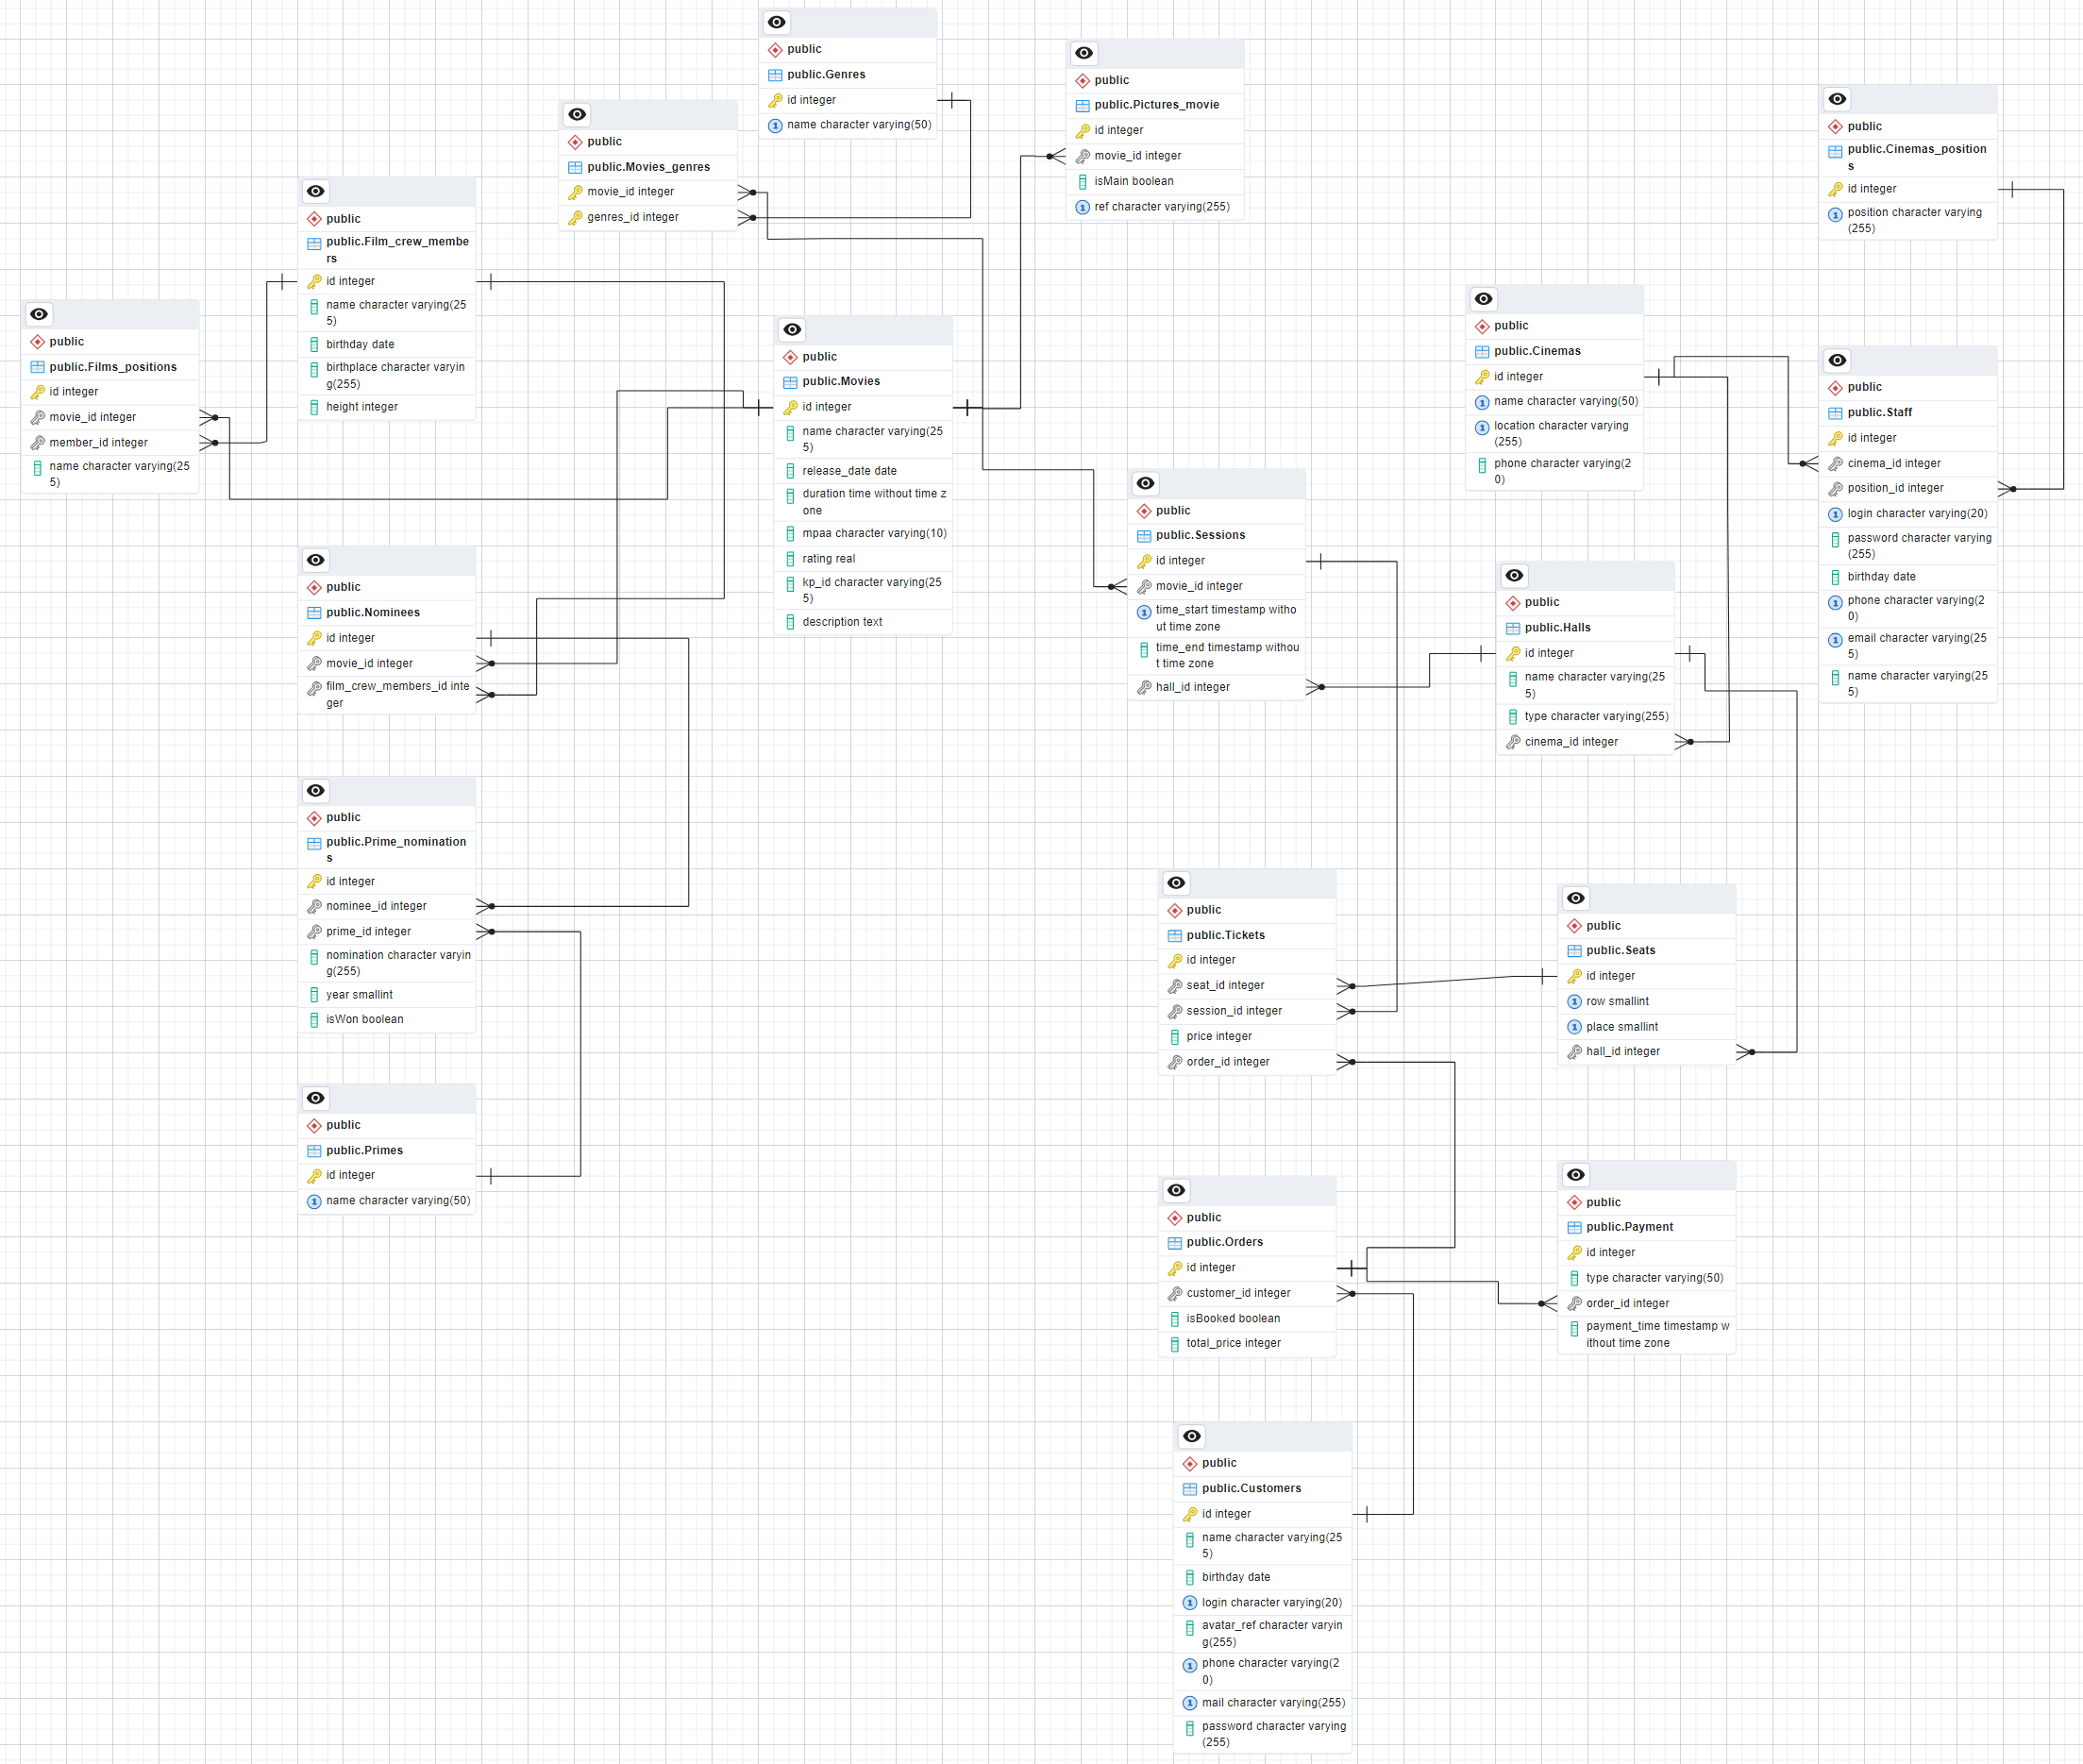
\includegraphics[scale=0.5,page=1]{Графическое представление.png}
		\caption{Графическое представление базы данных}
	\end{figure}
	
	\newpage
	
	\subsection{Создание таблиц}	
	
	Ниже приведены скриптовый код на языке SQL (диалект PostgreSQL) для создания таблиц, описанных выше.
	
	\begin{itemize}
	
	\lstdefinestyle{vscode-dark}{
		backgroundcolor=\color{black},
		basicstyle=\color{white}\ttfamily\tiny,
		breakatwhitespace=false,
		breaklines=true,
		captionpos=b,
		commentstyle=\color{green!40!black},
		keywordstyle=\color{cyan},
		numbersep=5pt,
		numberstyle=\tiny\color{gray},
		showstringspaces=false,
		stringstyle=\color{orange},
		tabsize=4
	}
	
	\item Код для создания таблицы Movies
		
	\begin{lstlisting}[style=vscode-dark, language=SQL, label={code:sql}]
		CREATE TABLE IF NOT EXISTS "public.Movies" (
			"id" serial NOT NULL,
			"name" varchar(255) NOT NULL,
			"release_date" DATE,
			"duration" TIME NOT NULL,
			"mpaa" varchar(10),
			"rating" float4,
			"kp_id" varchar(255),
			"description" TEXT,
			CONSTRAINT "Movies_pk" PRIMARY KEY ("id")
		) WITH (
			OIDS=FALSE
		);
	\end{lstlisting}


	\item Код для создания таблицы Genres

	\begin{lstlisting}[style=vscode-dark, language=SQL, label={code:sql}]
		CREATE TABLE IF NOT EXISTS "public.Genres" (
			"id" serial NOT NULL,
			"name" varchar(50) UNIQUE NOT NULL,
		CONSTRAINT "Genres_pk" PRIMARY KEY ("id")
		) WITH (
			OIDS=FALSE
		);
	\end{lstlisting}

	\item Код для создания таблицы Movies\_genres

	\begin{lstlisting}[style=vscode-dark, language=SQL, label={code:sql}]
		CREATE TABLE IF NOT EXISTS "public.Movies_genres" (
			"movie_id" integer NOT NULL,
			"genres_id" integer NOT NULL,
			CONSTRAINT "Movies_genres_pk" PRIMARY KEY ("movie_id", "genres_id")
		) WITH (
			OIDS=FALSE
		);
		
		ALTER TABLE "public.Movies_genres" ADD CONSTRAINT "Movies_genres_fk0" FOREIGN KEY ("movie_id") REFERENCES "public.Movies"("id");
		ALTER TABLE "public.Movies_genres" ADD CONSTRAINT "Movies_genres_fk1" FOREIGN KEY ("genres_id") REFERENCES "public.Genres"("id");
	\end{lstlisting}

	\item Код для создания таблицы Pictures\_movie

	\begin{lstlisting}[style=vscode-dark, language=SQL, label={code:sql}]
		CREATE TABLE IF NOT EXISTS "public.Pictures_movie" (
			"id" serial NOT NULL,
			"movie_id" integer NOT NULL,
			"isMain" BOOLEAN NOT NULL DEFAULT 'false',
			"ref" varchar(255) NOT NULL UNIQUE,
			CONSTRAINT "Pictures_movie_pk" PRIMARY KEY ("id")
		) WITH (
			OIDS=FALSE
		);
		
		ALTER TABLE "public.Pictures_movie" ADD CONSTRAINT "Pictures_movie_fk0" FOREIGN KEY ("movie_id") REFERENCES "public.Movies"("id");
	\end{lstlisting}
	$\\$
	
	\item Код для создания таблицы Film\_crew\_members
	
	\begin{lstlisting}[style=vscode-dark, language=SQL, label={code:sql}]
		CREATE TABLE IF NOT EXISTS "public.Film_crew_members" (
			"id" serial NOT NULL,
			"name" varchar(255) NOT NULL,
			"birthday" DATE,
			"birthplace" varchar(255),
			"height" integer,
			CONSTRAINT "Film_crew_members_pk" PRIMARY KEY ("id")
		) WITH (
			OIDS=FALSE
		);
	\end{lstlisting}

	\item Код для создания таблицы Films\_positions

	\begin{lstlisting}[style=vscode-dark, language=SQL, label={code:sql}]
		CREATE TABLE IF NOT EXISTS "public.Films_positions" (
			"id" serial NOT NULL,
			"movie_id" integer NOT NULL,
			"member_id" integer NOT NULL,
			"name" varchar(255) NOT NULL,
			CONSTRAINT "Films_crews_pk" PRIMARY KEY ("id")
		) WITH (
			OIDS=FALSE
		);
		
		ALTER TABLE "public.Films_positions" ADD CONSTRAINT "Films_positions_fk0" FOREIGN KEY ("movie_id") REFERENCES "public.Movies"("id");
		ALTER TABLE "public.Films_positions" ADD CONSTRAINT "Films_positions_fk1" FOREIGN KEY ("member_id") REFERENCES "public.Film_crew_members"("id");
	\end{lstlisting}
	
	\item Код для создания таблицы Nominees
	
	\begin{lstlisting}[style=vscode-dark, language=SQL, label={code:sql}]
		CREATE TABLE IF NOT EXISTS "public.Nominees" (
			"id" serial NOT NULL,
			"movie_id" integer,
			"film_crew_members_id" integer,
			CONSTRAINT "Nominees_pk" PRIMARY KEY ("id")
		) WITH (
			OIDS=FALSE
		);
		
		ALTER TABLE "public.Nominees" ADD CONSTRAINT "Nominees_fk0" FOREIGN KEY ("movie_id") REFERENCES "public.Movies"("id");
		ALTER TABLE "public.Nominees" ADD CONSTRAINT "Nominees_fk1" FOREIGN KEY ("film_crew_members_id") REFERENCES "public.Film_crew_members"("id");
		ALTER TABLE "public.Nominees" ADD CONSTRAINT "Nominees_unique" UNIQUE("movie_id","film_crew_members_id");
	\end{lstlisting}
	
	\item Код для создания таблицы Primes
	
	\begin{lstlisting}[style=vscode-dark, language=SQL, label={code:sql}]
		CREATE TABLE IF NOT EXISTS "public.Primes" (
			"id" serial NOT NULL,
			"name" varchar(50) NOT NULL UNIQUE,
			CONSTRAINT "Primes_pk" PRIMARY KEY ("id")
		) WITH (
			OIDS=FALSE
		);
	\end{lstlisting}

	\item Код для создания таблицы Prime\_nominations

	\begin{lstlisting}[style=vscode-dark, language=SQL, label={code:sql}]
		CREATE TABLE IF NOT EXISTS "public.Prime_nominations" (
			"id" serial NOT NULL,
			"nominee_id" integer NOT NULL,
			"prime_id" integer NOT NULL,
			"nomination" varchar(255) NOT NULL,
			"year" smallint NOT NULL,
			"isWon" BOOLEAN NOT NULL DEFAULT 'false',
			CONSTRAINT "Prime_nominations_pk" PRIMARY KEY ("id")
		) WITH (
			OIDS=FALSE
		);
		
		ALTER TABLE "public.Prime_nominations" ADD CONSTRAINT "Prime_nominations_fk0" FOREIGN KEY ("nominee_id") REFERENCES "public.Nominees"("id");
		ALTER TABLE "public.Prime_nominations" ADD CONSTRAINT "Prime_nominations_fk1" FOREIGN KEY ("prime_id") REFERENCES "public.Primes"("id");
	\end{lstlisting}
	
	\item Код для создания таблицы Cinemas
	
	\begin{lstlisting}[style=vscode-dark, language=SQL, label={code:sql}]
		CREATE TABLE IF NOT EXISTS "public.Cinemas" (
			"id" serial NOT NULL,
			"name" varchar(50) NOT NULL UNIQUE,
			"location" varchar(255) UNIQUE,
			"phone" varchar(20),
			CONSTRAINT "Cinemas_pk" PRIMARY KEY ("id")
		) WITH (
			OIDS=FALSE
		);
	\end{lstlisting}
	
	\item Код для создания таблицы Halls
	
	\begin{lstlisting}[style=vscode-dark, language=SQL, label={code:sql}]
		CREATE TABLE IF NOT EXISTS "public.Halls" (
			"id" serial NOT NULL,
			"name" varchar(255) NOT NULL,
			"type" varchar(255),
			"cinema_id" integer NOT NULL,
			CONSTRAINT "Halls_pk" PRIMARY KEY ("id")
		) WITH (
			OIDS=FALSE
		);
		
		ALTER TABLE "public.Halls" ADD CONSTRAINT "Halls_fk0" FOREIGN KEY ("cinema_id") REFERENCES "public.Cinemas"("id");
	\end{lstlisting}

	\item Код для создания таблицы Sessions

	\begin{lstlisting}[style=vscode-dark, language=SQL, label={code:sql}]
		CREATE TABLE IF NOT EXISTS "public.Sessions" (
			"id" serial NOT NULL,
			"movie_id" serial NOT NULL ,
			"time_start" TIMESTAMP NOT NULL,
			"time_end" TIMESTAMP NOT NULL,
			"hall_id" integer NOT NULL,
			CONSTRAINT "Sessions_pk" PRIMARY KEY ("id")
		) WITH (
			OIDS=FALSE
		);
		
		ALTER TABLE "public.Sessions" ADD CONSTRAINT "Sessions_fk0" FOREIGN KEY ("movie_id") REFERENCES "public.Movies"("id");
		ALTER TABLE "public.Sessions" ADD CONSTRAINT "Sessions_fk1" FOREIGN KEY ("hall_id") REFERENCES "public.Halls"("id");
		ALTER TABLE "public.Sessions" ADD CONSTRAINT "Sessions_unique" UNIQUE("hall_id", "time_start");
	\end{lstlisting}
	
	\item Код для создания таблицы Seats
	
	\begin{lstlisting}[style=vscode-dark, language=SQL, label={code:sql}]
		CREATE TABLE IF NOT EXISTS "public.Seats" (
			"id" serial NOT NULL,
			"row" smallint NOT NULL,
			"place" smallint NOT NULL,
			"hall_id" integer NOT NULL,
			CONSTRAINT "Seats_pk" PRIMARY KEY ("id")
		) WITH (
			OIDS=FALSE
		);
		
		ALTER TABLE "public.Seats" ADD CONSTRAINT "Seats_fk0" FOREIGN KEY ("hall_id") REFERENCES "public.Halls"("id");
		ALTER TABLE "public.Seats" ADD CONSTRAINT "Seats_unique" UNIQUE("row", "place", "hall_id");
	\end{lstlisting}

	\item Код для создания таблицы Customers

	\begin{lstlisting}[style=vscode-dark, language=SQL, label={code:sql}]
		CREATE TABLE IF NOT EXISTS "public.Customers" (
			"id" serial NOT NULL,
			"name" varchar(255),
			"birthday" DATE,
			"login" varchar(20) UNIQUE,
			"avatar_ref" varchar(255),
			"phone" varchar(20) UNIQUE,
			"mail" varchar(255) UNIQUE,
			"password" varchar(255) NOT NULL,
			CONSTRAINT "Customers_pk" PRIMARY KEY ("id")
		) WITH (
			OIDS=FALSE
		);
	\end{lstlisting}

	\item Код для создания таблицы Orders

	\begin{lstlisting}[style=vscode-dark, language=SQL, label={code:sql}]
		CREATE TABLE IF NOT EXISTS "public.Orders" (
			"id" serial NOT NULL,
			"customer_id" integer NOT NULL,
			"isBooked" BOOLEAN DEFAULT(false),
			"total_price" integer NOT NULL DEFAULT 0,
			CONSTRAINT "Orders_pk" PRIMARY KEY ("id")
		) WITH (
			OIDS=FALSE
		);
		
		ALTER TABLE "public.Orders" ADD CONSTRAINT "Orders_fk0" FOREIGN KEY ("customer_id") REFERENCES "public.Customers"("id");
	\end{lstlisting}
	
	\item Код для создания таблицы Payment

	\begin{lstlisting}[style=vscode-dark, language=SQL, label={code:sql}]
		CREATE TABLE IF NOT EXISTS "public.Payment" (
			"id" serial NOT NULL,
			"type" varchar(50) NOT NULL,
			"order_id" integer NOT NULL UNIQUE,
			"payment_time" TIMESTAMP,
			CONSTRAINT "Payment_pk" PRIMARY KEY ("id")
		) WITH (
			OIDS=FALSE
		);
		
		ALTER TABLE "public.Payment"  ADD CONSTRAINT "Payment_fk0" FOREIGN KEY ("order_id") REFERENCES "public.Orders"("id");
	\end{lstlisting}

	\item Код для создания таблицы Tickets

	\begin{lstlisting}[style=vscode-dark, language=SQL, label={code:sql}]
		CREATE TABLE IF NOT EXISTS "public.Tickets" (
			"id" serial NOT NULL,
			"seat_id" integer NOT NULL,
			"session_id" integer NOT NULL,
			"price" integer NOT NULL,
			"order_id" integer NOT NULL,
			CONSTRAINT "Tickets_pk" PRIMARY KEY ("id")
		) WITH (
			OIDS=FALSE
		);
		
		ALTER TABLE "public.Tickets" ADD CONSTRAINT "Tickets_fk0" FOREIGN KEY ("seat_id") REFERENCES "public.Seats"("id");
		ALTER TABLE "public.Tickets" ADD CONSTRAINT "Tickets_fk1" FOREIGN KEY ("session_id") REFERENCES "public.Sessions"("id");
		ALTER TABLE "public.Tickets" ADD CONSTRAINT "Tickets_fk2" FOREIGN KEY ("order_id") REFERENCES "public.Orders"("id");
		ALTER TABLE "public.Tickets" ADD CONSTRAINT "Tickets_unique" UNIQUE("seat_id", "session_id");
	\end{lstlisting}

	\item Код для создания таблицы Cinemas\_positions

	\begin{lstlisting}[style=vscode-dark, language=SQL, label={code:sql}]
		CREATE TABLE IF NOT EXISTS "public.Cinemas_positions" (
			"id" serial NOT NULL,
			"position" varchar(255) NOT NULL UNIQUE,
			CONSTRAINT "Cinemas_positions_pk" PRIMARY KEY ("id")
		) WITH (
			OIDS=FALSE
		);
	\end{lstlisting}
	
	\item Код для создания таблицы Staff
	
	\begin{lstlisting}[style=vscode-dark, language=SQL, label={code:sql}]
		CREATE TABLE IF NOT EXISTS "public.Staff" (
			"id" serial NOT NULL,
			"cinema_id" integer NOT NULL,
			"position_id" integer NOT NULL,
			"login" varchar(20) NOT NULL UNIQUE,
			"password" varchar(255) NOT NULL,
			"birthday" DATE NOT NULL,
			"phone" varchar(20) NOT NULL UNIQUE,
			"email" varchar(255) NOT NULL UNIQUE,
			"name" varchar(255) NOT NULL,
		CONSTRAINT "Staff_pk" PRIMARY KEY ("id")
		) WITH (
			OIDS=FALSE
		);
		
		ALTER TABLE "public.Staff" ADD CONSTRAINT "Staff_fk0" FOREIGN KEY ("cinema_id") REFERENCES "public.Cinemas"("id");
		ALTER TABLE "public.Staff" ADD CONSTRAINT "Staff_fk1" FOREIGN KEY ("position_id") REFERENCES "public.Cinemas_positions"("id");
	\end{lstlisting}

	\end{itemize}
		
		
	\newpage
	
	\subsection{Заполнение базы данных}
	
	%\newpage
	
	\subsubsection{Подготовка данных}
	
	В сети Интернет найдены такие данные как существующие жанры фильмов, существующие награды и номинации к фильмам. Такие данные как сведения о фильмах (название, дата выхода, длительность, описание), сведения об актёрах (имя, дата рождения, место рождения, рост), сведения о пользователях и сотрудниках (имя, дата рождения, логин, пароль, телефон, почта, ссылка на аватар) были сгенерированы Pyhton библиотекой Faker. Для предварительной оценки сгенерированных данных они были вносились в Excel-таблицы, которые после импортировались в Python с использованием библиотеки Pandas и использовались в автоматизированном написании нужных запросов для заполнения таблиц.
	
	\begin{itemize}
	
	\item Фрагмент сгенерированной Excel-таблицы для заполнения Movies
	
	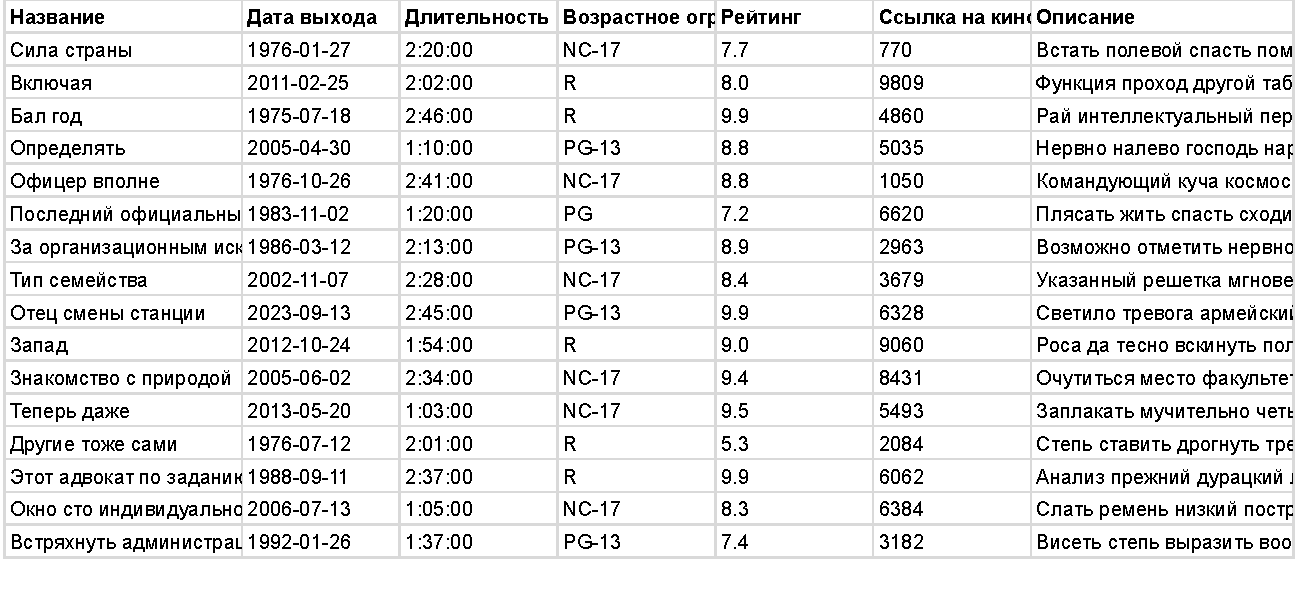
\includegraphics[scale=0.7,page=1]{movies_random.pdf}
	

	\item Фрагмент сгенерированной Excel-таблицы для заполнения Movies\_genres
	
	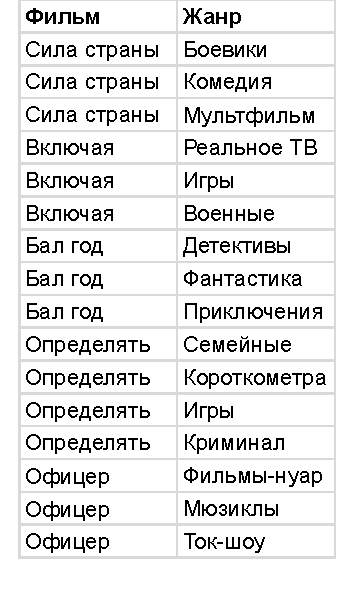
\includegraphics[scale=0.7,page=1]{movies_genres_random.pdf}
	

	\item Фрагмент сгенерированной Excel-таблицы для заполнения Pictures\_movie
	
	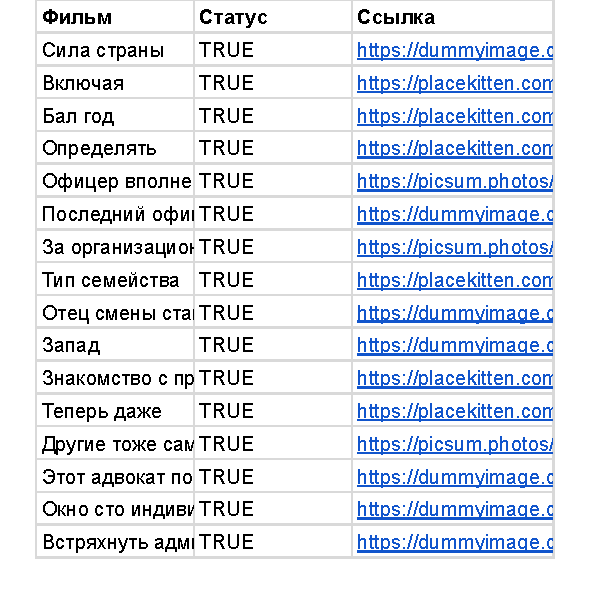
\includegraphics[scale=0.7,page=1]{movie_pictures_random.pdf}
	

	\item Фрагмент сгенерированной Excel-таблицы для заполнения Film\_crew\_members
	
	
	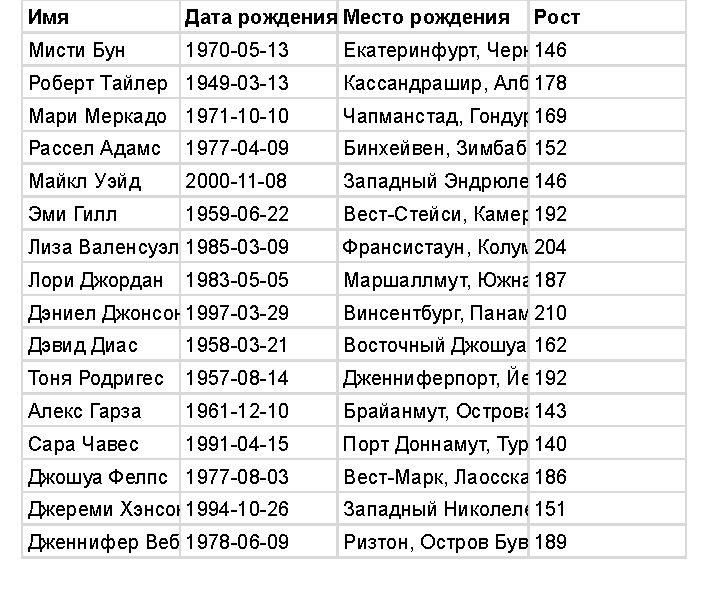
\includegraphics[scale=0.7,page=1]{members_random.pdf}
	

	\item Фрагмент сгенерированной Excel-таблицы для заполнения Films\_positions
	
	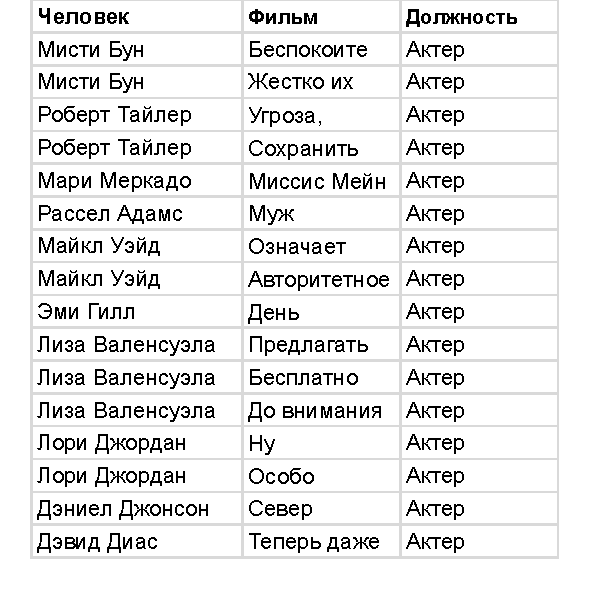
\includegraphics[scale=0.7,page=1]{members_movies_random.pdf}
	$\\$
	
	\item Фрагмент сгенерированной Excel-таблицы для заполнения Prime\_nominations
	
	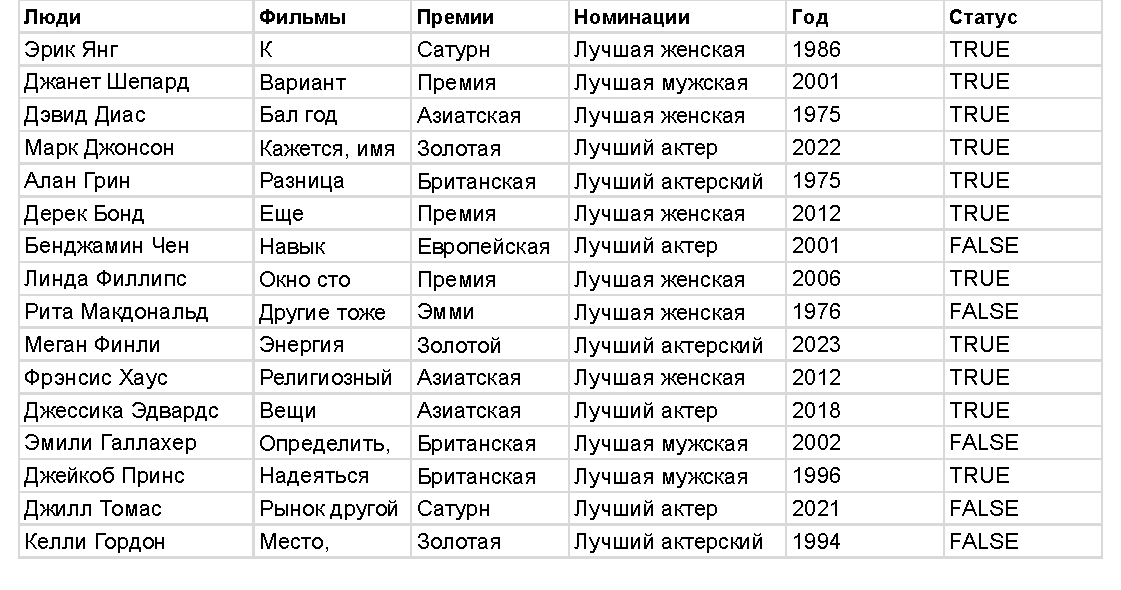
\includegraphics[scale=0.7,page=1]{prime_nominations_random.pdf}
	

	\item Фрагмент сгенерированной Excel-таблицы для заполнения Cinemas
	
	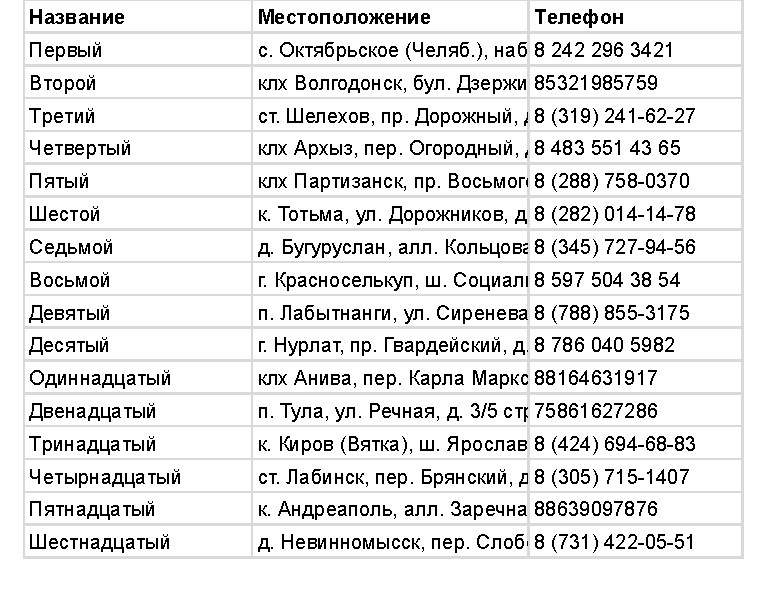
\includegraphics[scale=0.7,page=1]{cinemas_random.pdf}
	

	\item Фрагмент сгенерированной Excel-таблицы для заполнения Halls
	
	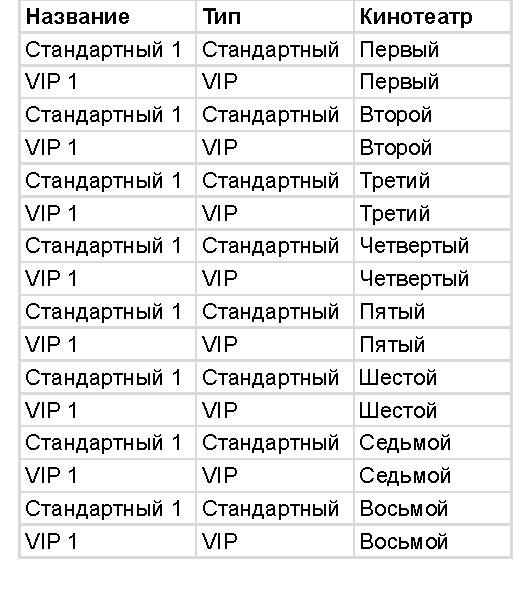
\includegraphics[scale=0.7,page=1]{halls_random.pdf}
	$\\$
	
	\item Фрагмент сгенерированной Excel-таблицы для заполнения Sessions
	
	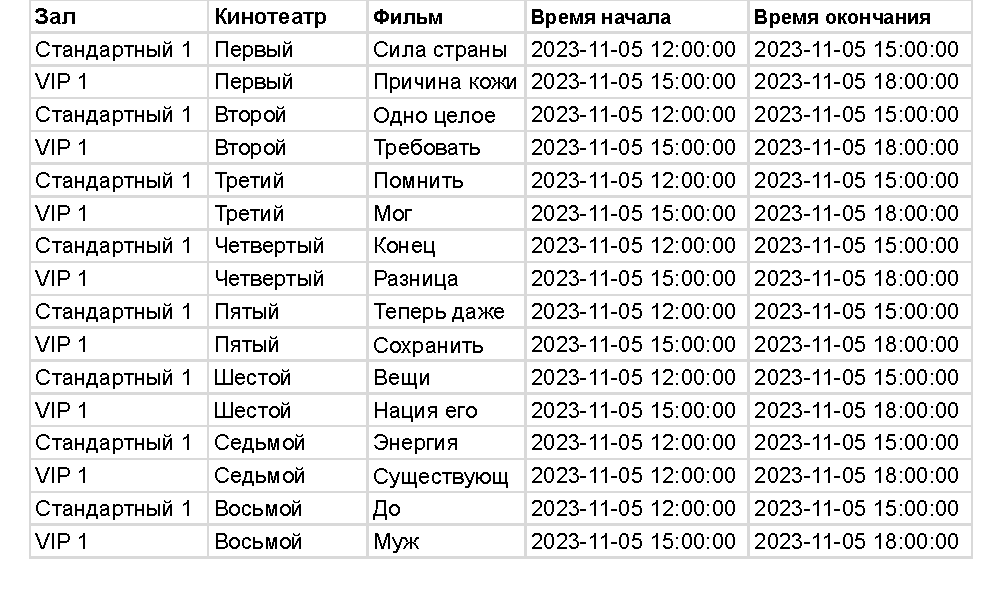
\includegraphics[scale=0.7,page=1]{sessions_random.pdf}
	
	
	\item Фрагмент сгенерированной Excel-таблицы для заполнения Customers
	
	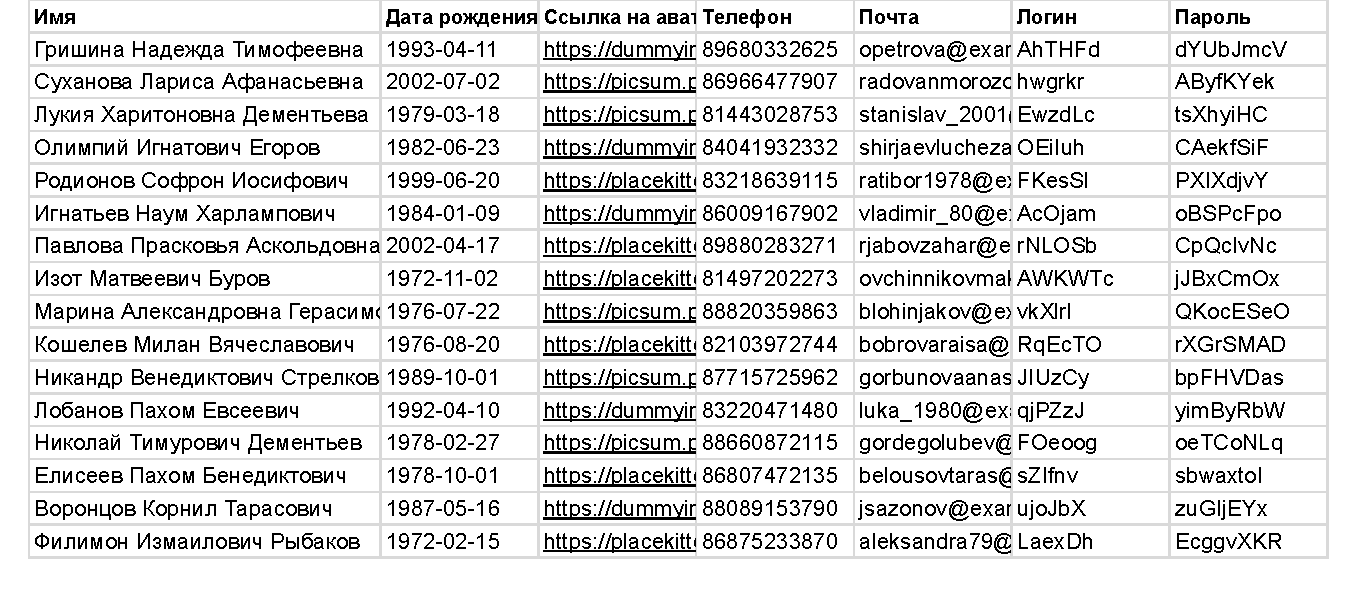
\includegraphics[scale=0.7,page=1]{customers_random.pdf}
	
	
	\item Фрагмент сгенерированной Excel-таблицы для заполнения Payment
	
	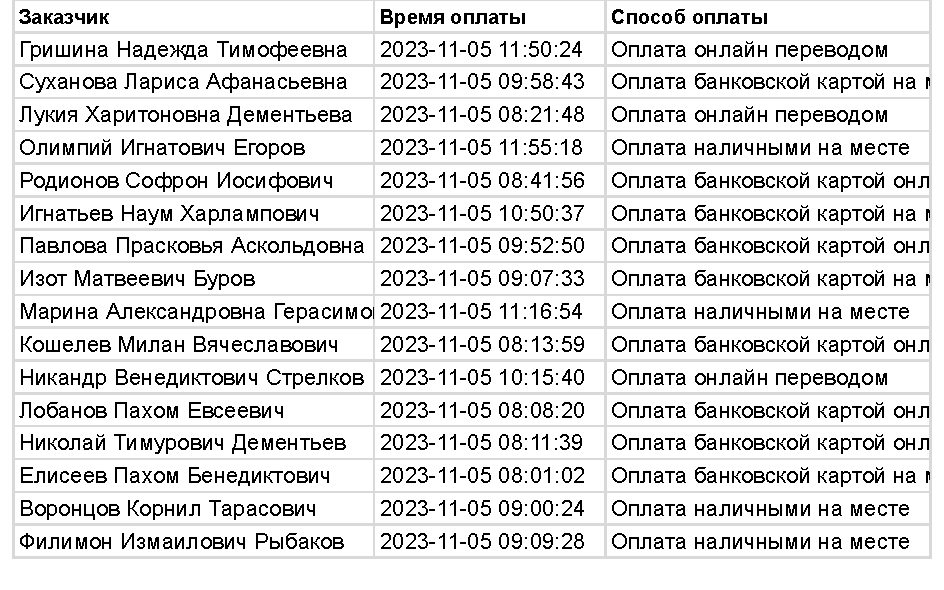
\includegraphics[scale=0.7,page=1]{payment_random.pdf}
	$\\$
	
	
	\item Фрагмент сгенерированной Excel-таблицы для заполнения Tickets
	
	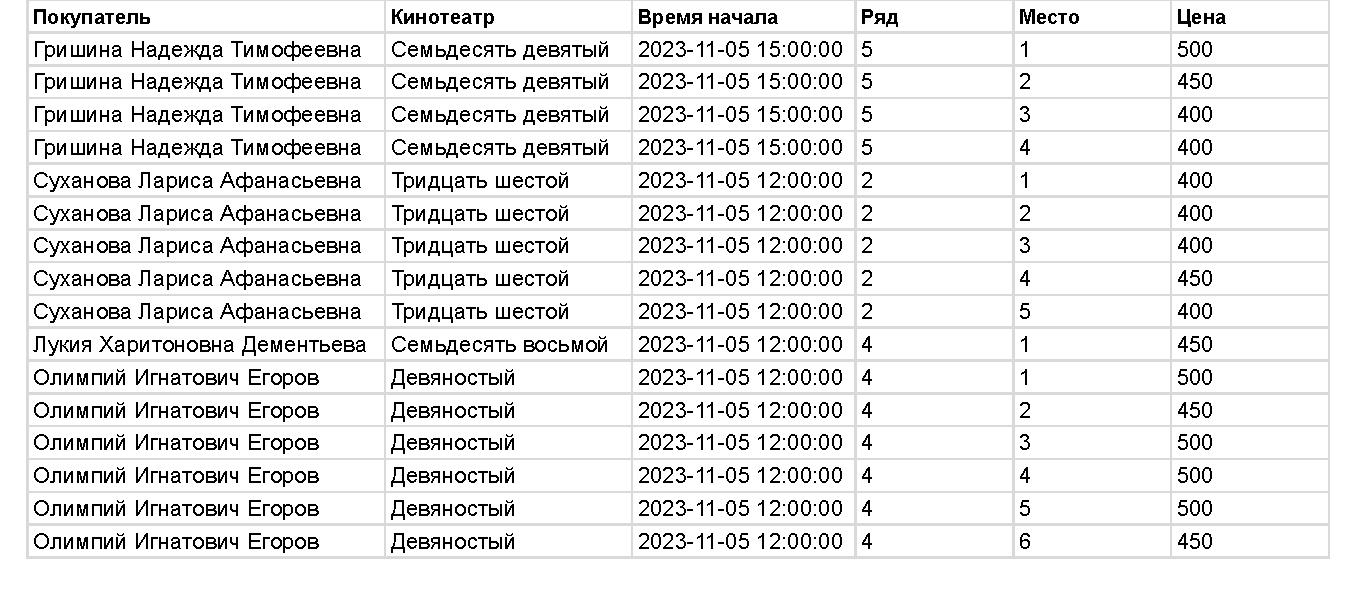
\includegraphics[scale=0.7,page=1]{tickets_random.pdf}
	
	
	\item Фрагмент сгенерированной Excel-таблицы для заполнения Staff
	
	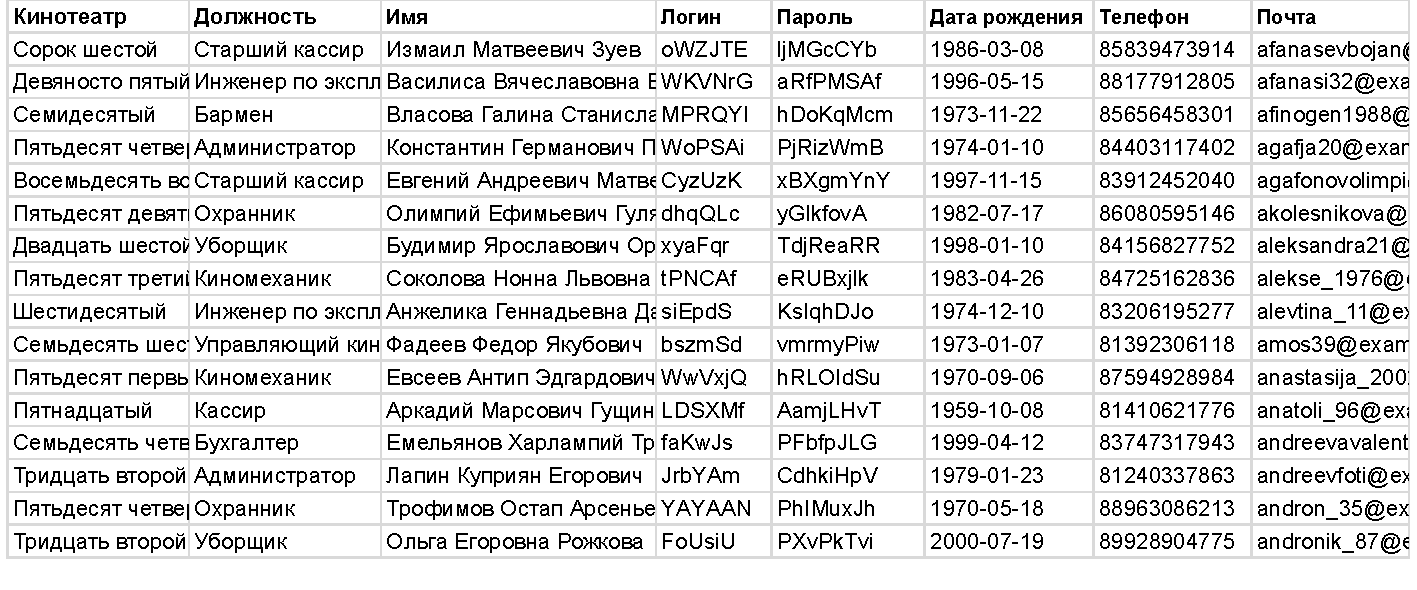
\includegraphics[scale=0.7,page=1]{staff_random.pdf}
	
	\end{itemize}
	
	\newpage
	
	\subsubsection{Программа заполнения базы данных}
	
	Ниже приведён пример Python-кода, который принимает данные из Excel-таблицы и генерирует SQL-запрос на заполнение данными таблицы Tickets.
	
	\begin{figure}[h]
		\hspace{-0.5cm}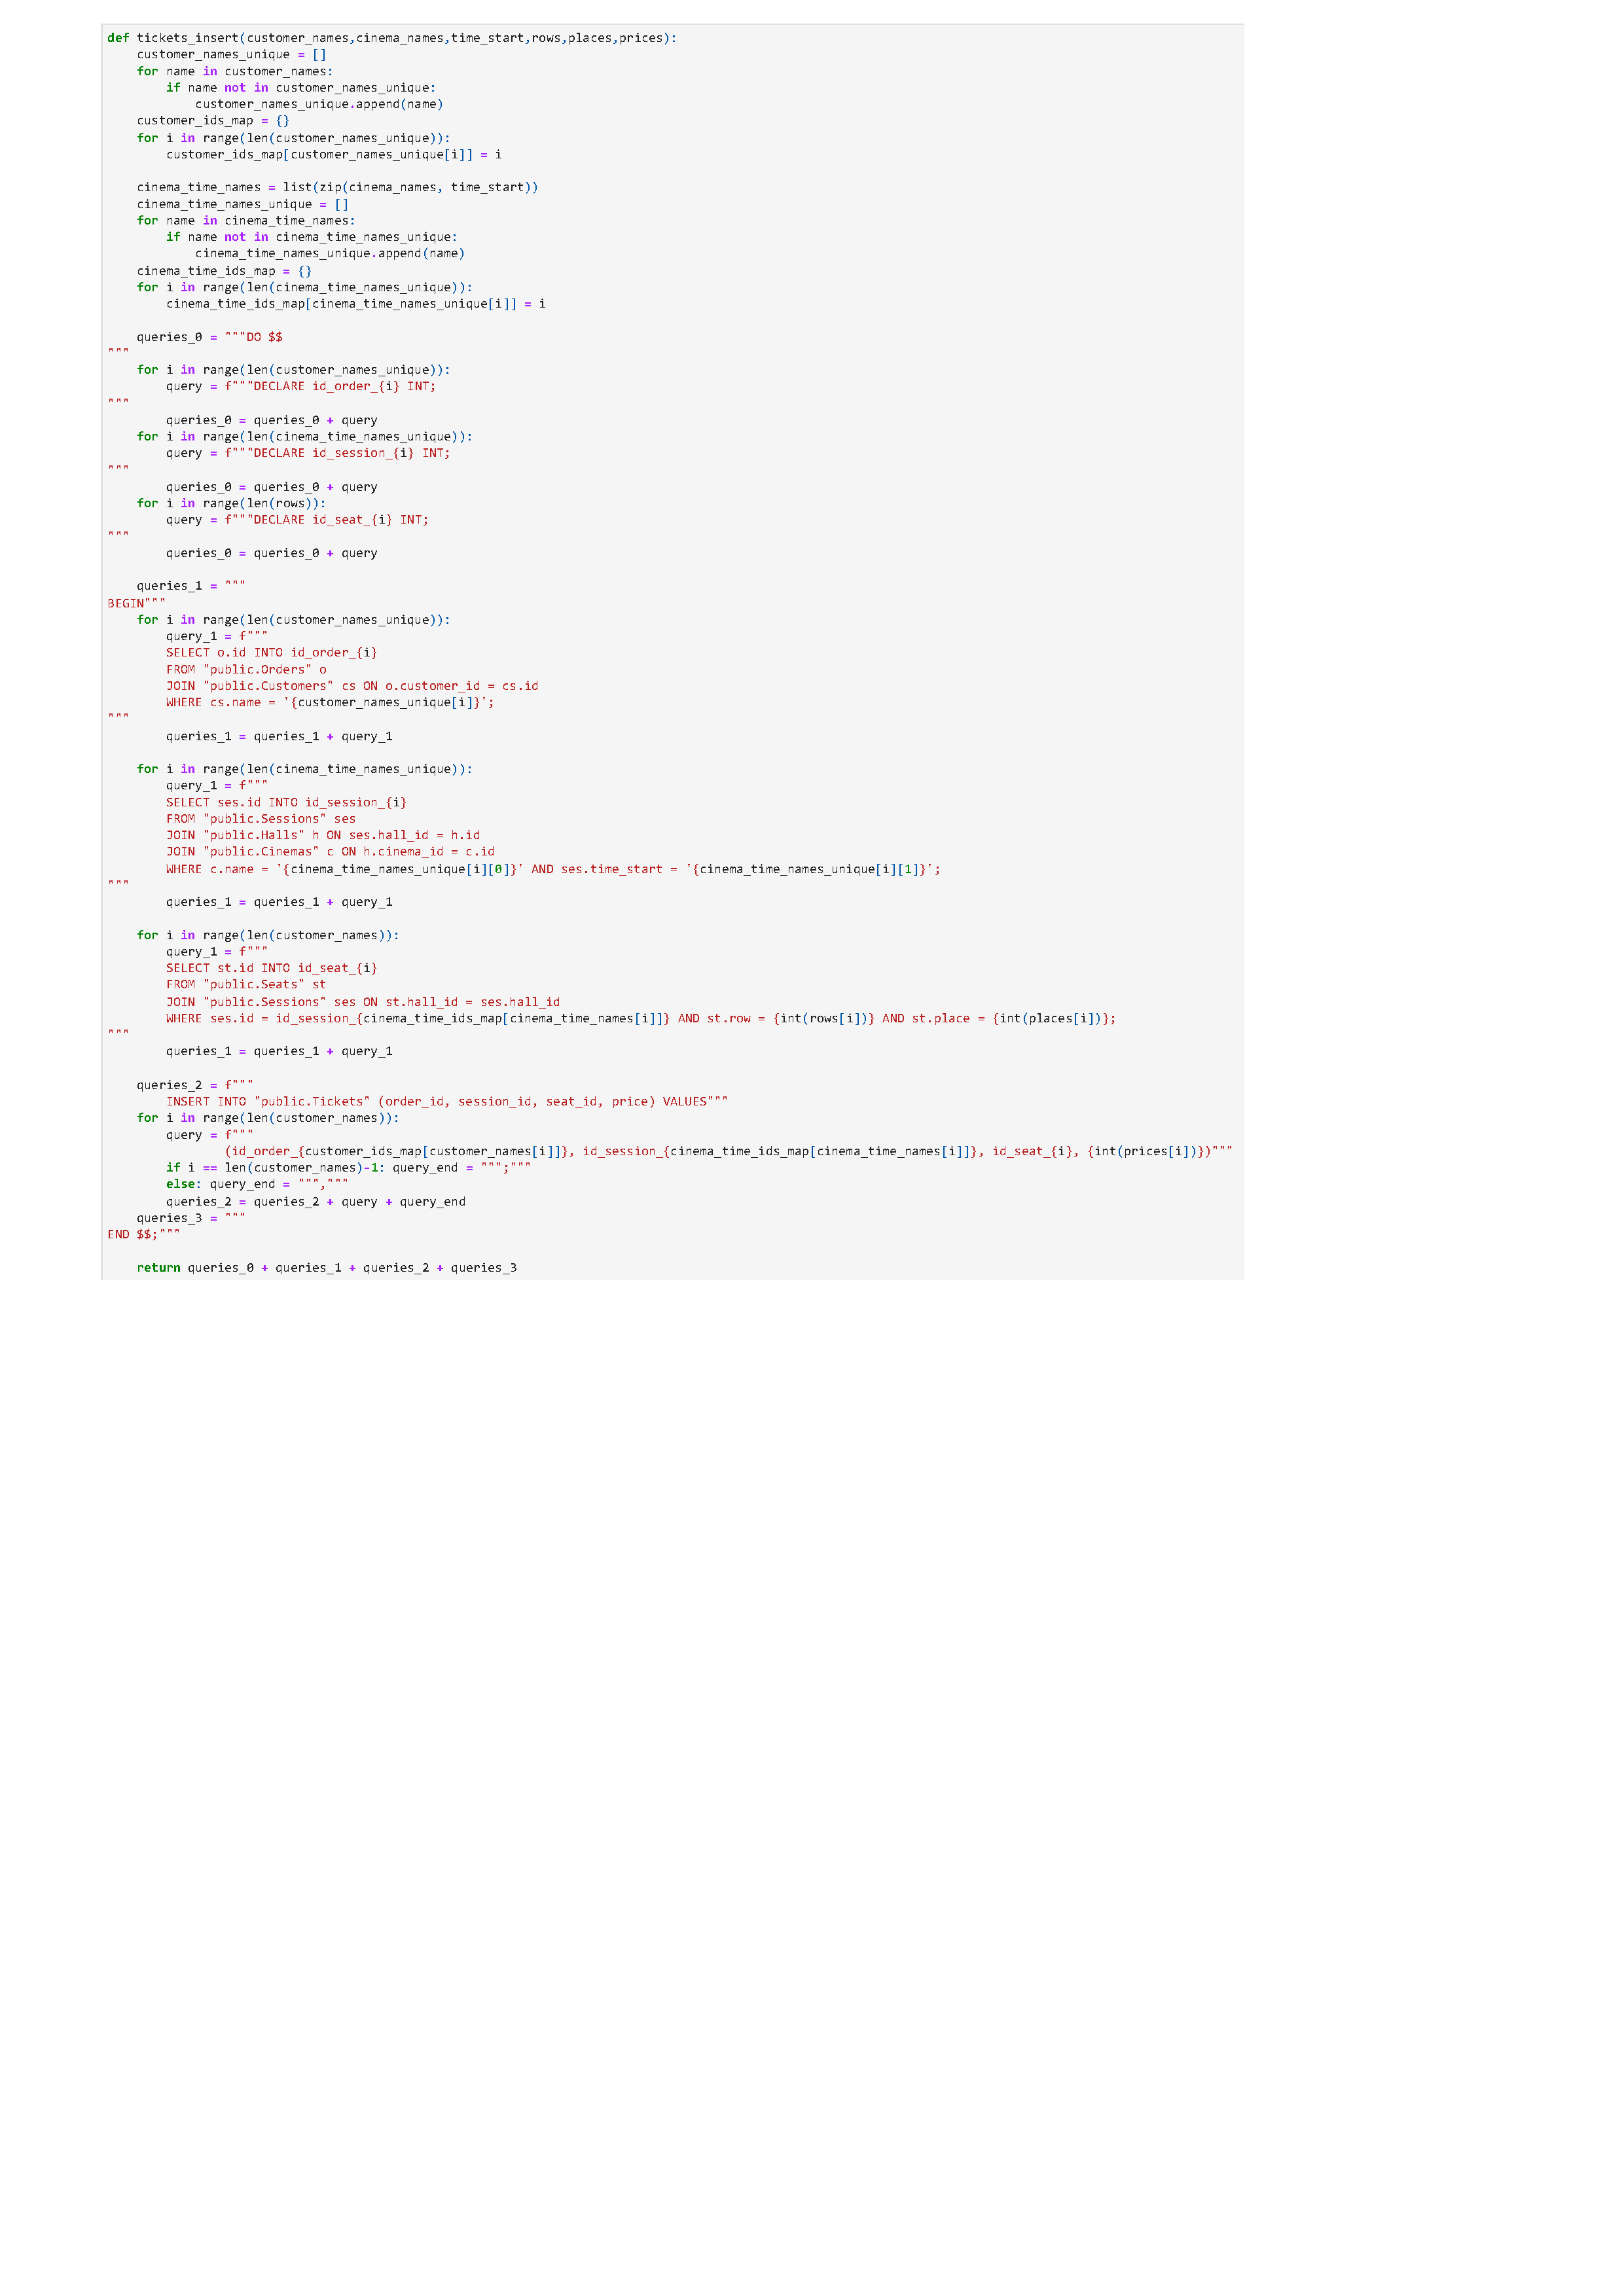
\includegraphics[scale=0.6,page=1]{sql_tickets_insert.pdf}
	\end{figure}

	Все генерируемые подобным образом SQL-запросы направлены на то, чтобы искать id нужных таблиц и заполнять нужные данные на основе данных из Excel-таблиц. Причём нужные id в таком запросе ищутся ровно один раз даже в случае, если в Excel-таблице на один и тот же id ссылаются несколько раз.
	
	\newpage
	
	\subsubsection{Результаты заполнения}
	
	\begin{itemize}
		
	\item Таблица Movies

	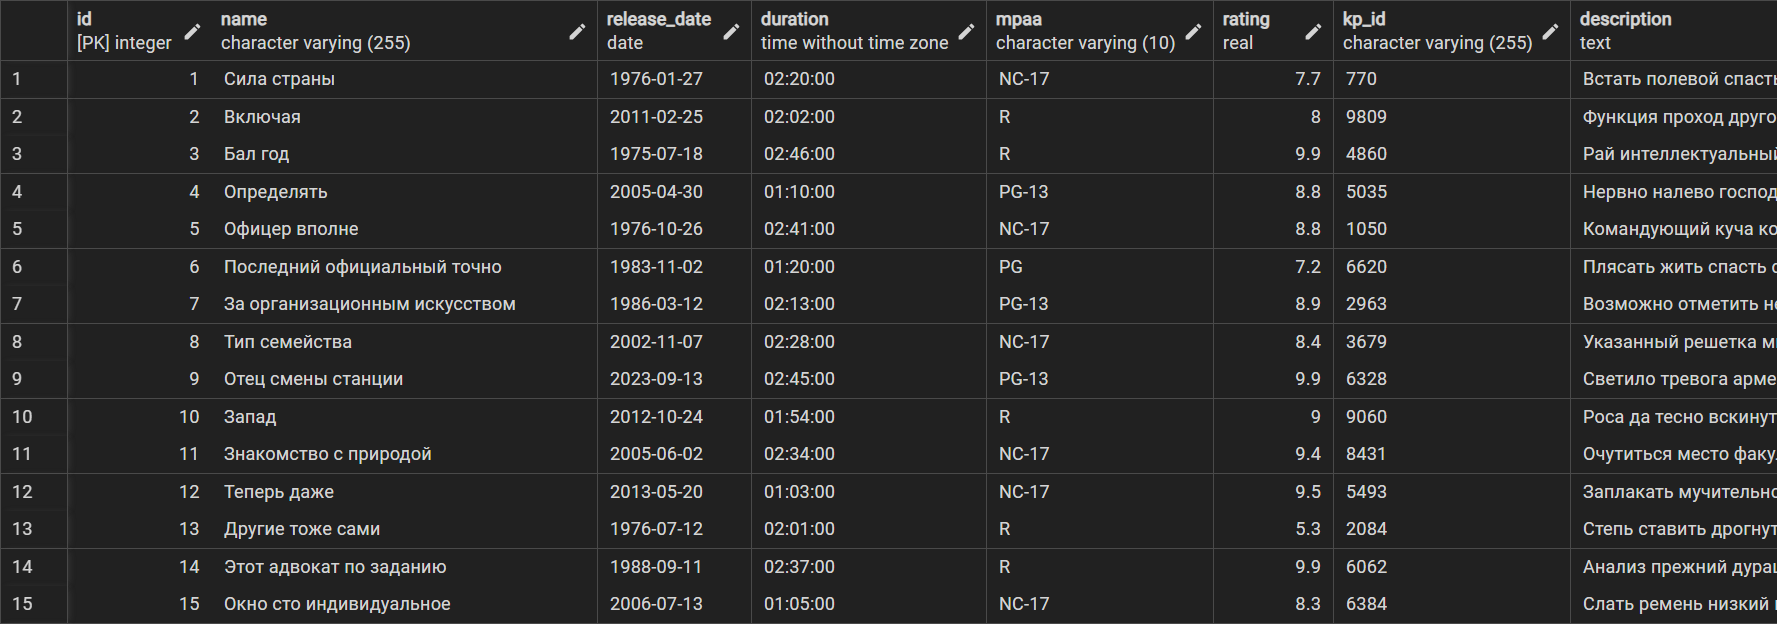
\includegraphics[scale=0.55,page=1]{Movies.png}
	
	
	\item Таблица Genres
	
	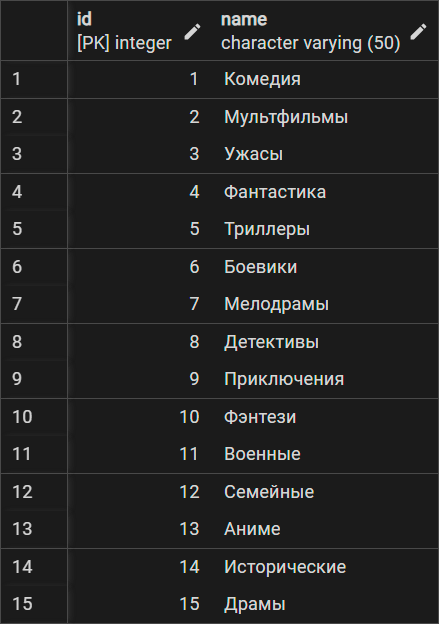
\includegraphics[scale=0.3,page=1]{Genres.png}
	
	
	\item Таблица Movies\_genres
	
	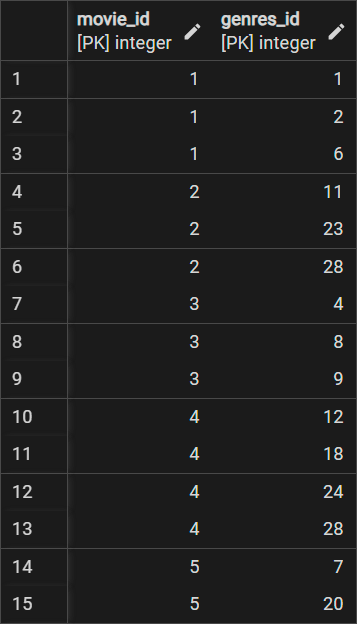
\includegraphics[scale=0.3,page=1]{Movies_genres.png}
	
	\newpage
	
	
	\item Таблица Pictures\_movie
	
	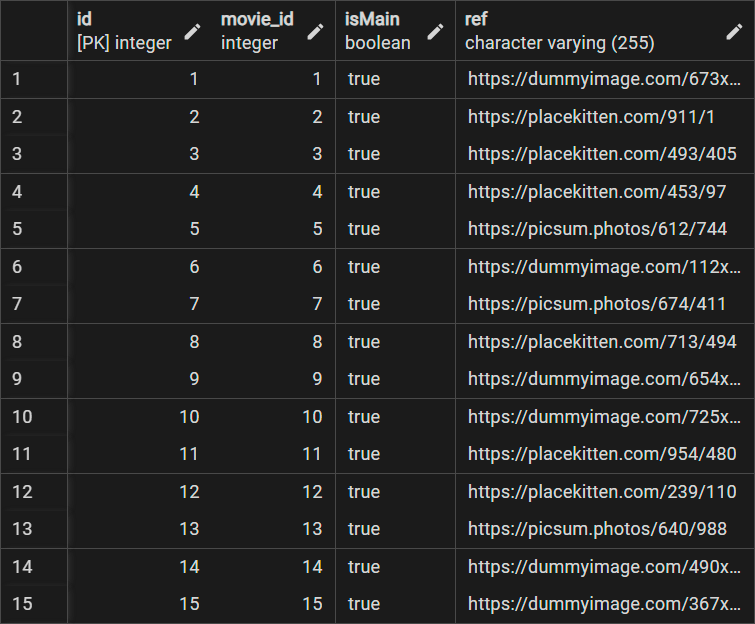
\includegraphics[scale=0.3,page=1]{Pictures_movie.png}
	
	
	\item Таблица Film\_crew\_members
	
	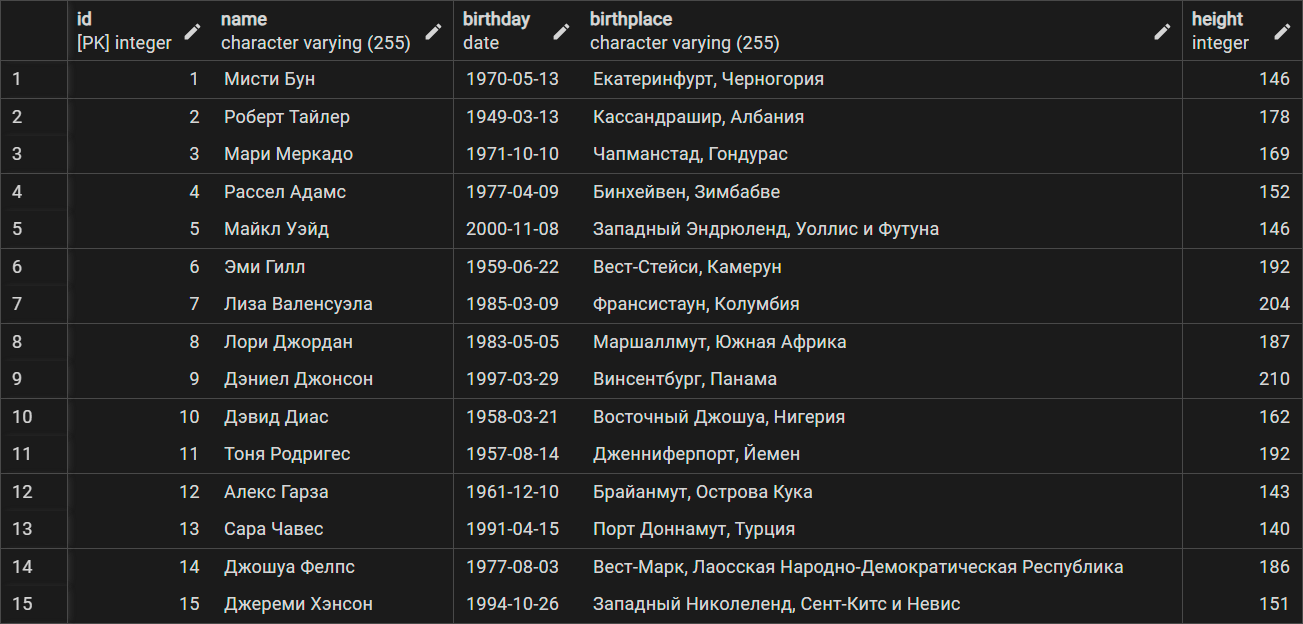
\includegraphics[scale=0.3,page=1]{Film_crew_members.png}
	
	
	\item Таблица Films\_positions
	
	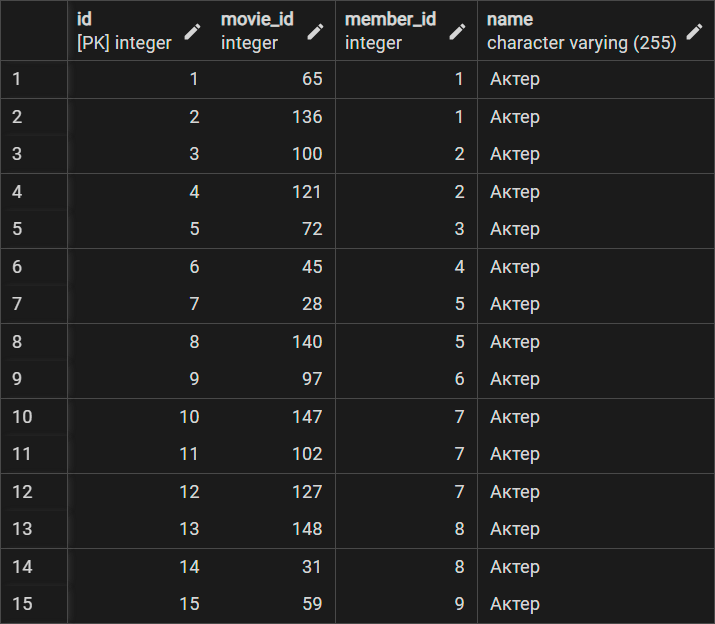
\includegraphics[scale=0.3,page=1]{Films_positions.png}
	
	\newpage
	
	\item Таблица Nominees
	
	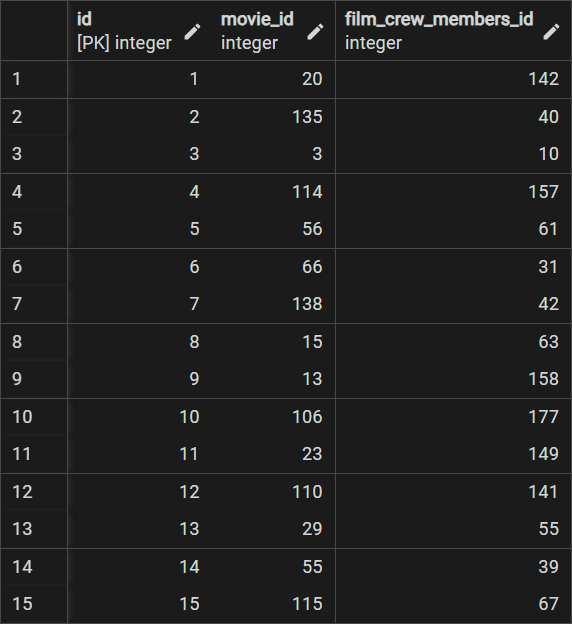
\includegraphics[scale=0.3,page=1]{Nominees.png}
	$\\$
	
	
	\item Таблица Primes
	
	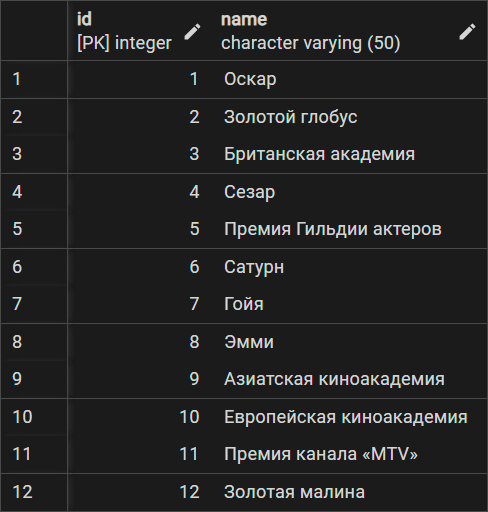
\includegraphics[scale=0.4,page=1]{Primes.png}
	$\\$
	
	
	\item Таблица Prime\_nominations
	
	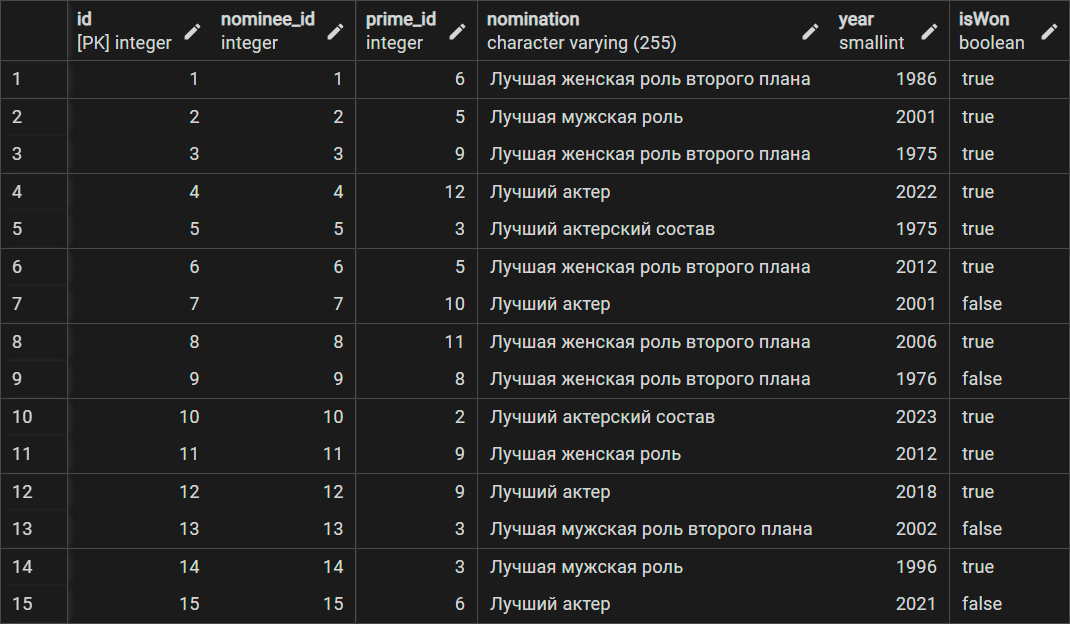
\includegraphics[scale=0.3,page=1]{Prime_nominations.png}

	
	
	\item Таблица Cinemas
	
	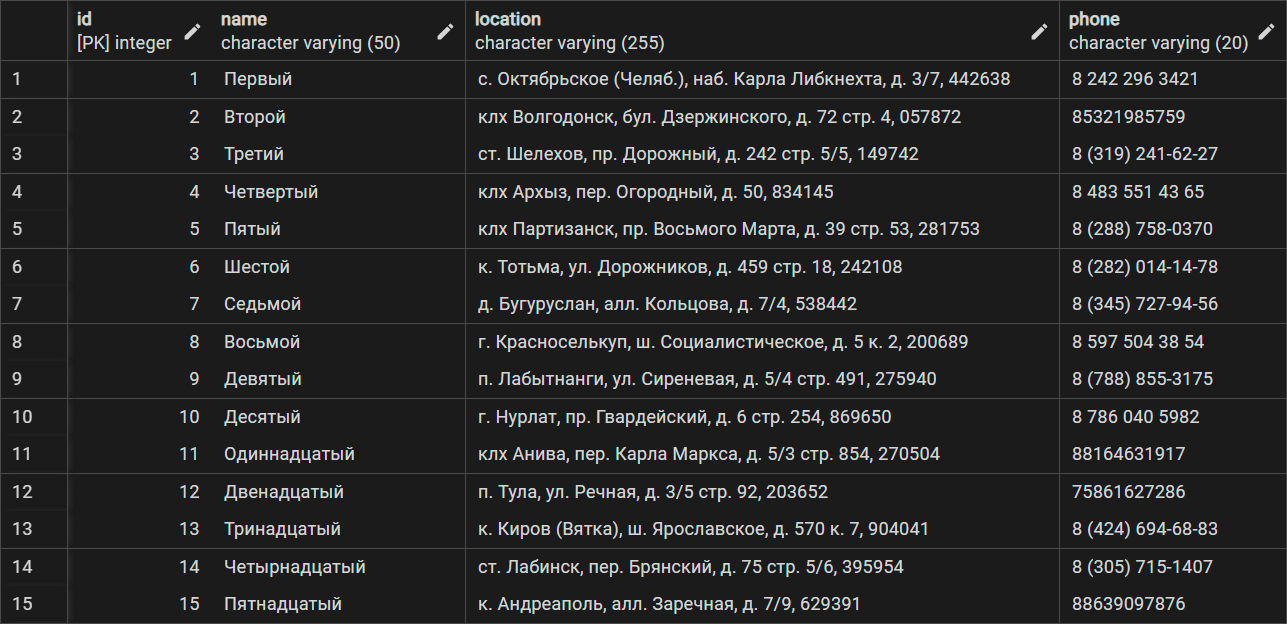
\includegraphics[scale=0.3,page=1]{Cinemas.png}
	$\\$
	
	
	\item Таблица Halls
	
	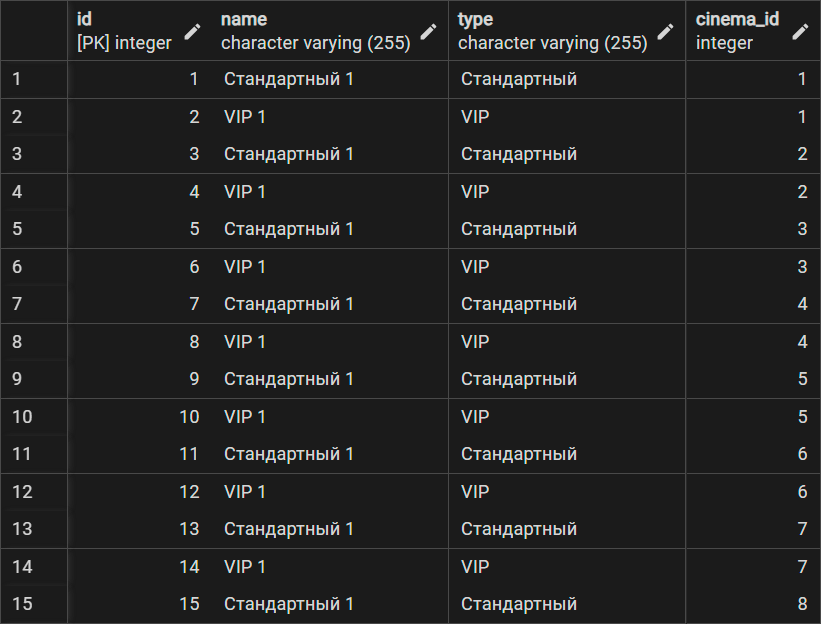
\includegraphics[scale=0.3,page=1]{Halls.png}
	$\\$
	
	
	\item Таблица Sessions
	
	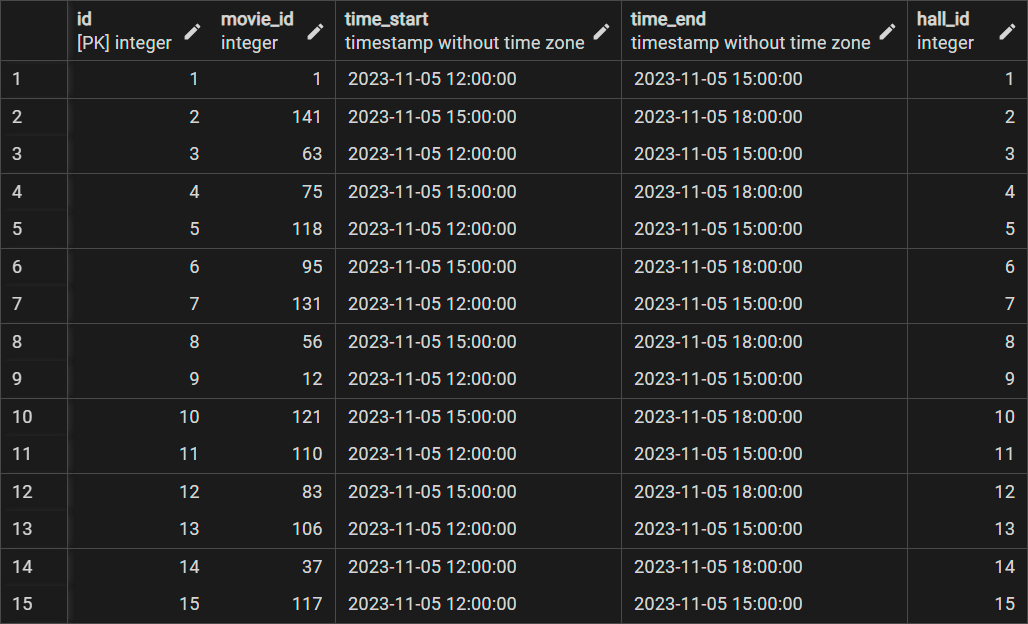
\includegraphics[scale=0.3,page=1]{Sessions.png}
	$\\$

	
	\item Таблица Seats
	
	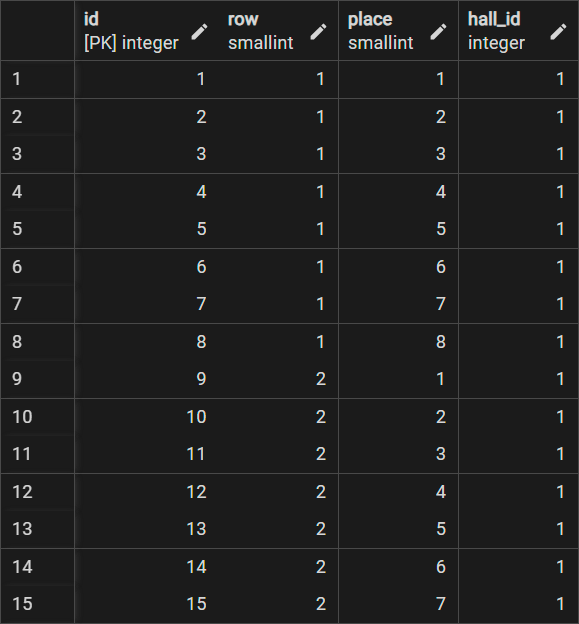
\includegraphics[scale=0.32,page=1]{Seats.png}
	$\\$
	
	
	\item Таблица Customers
	
	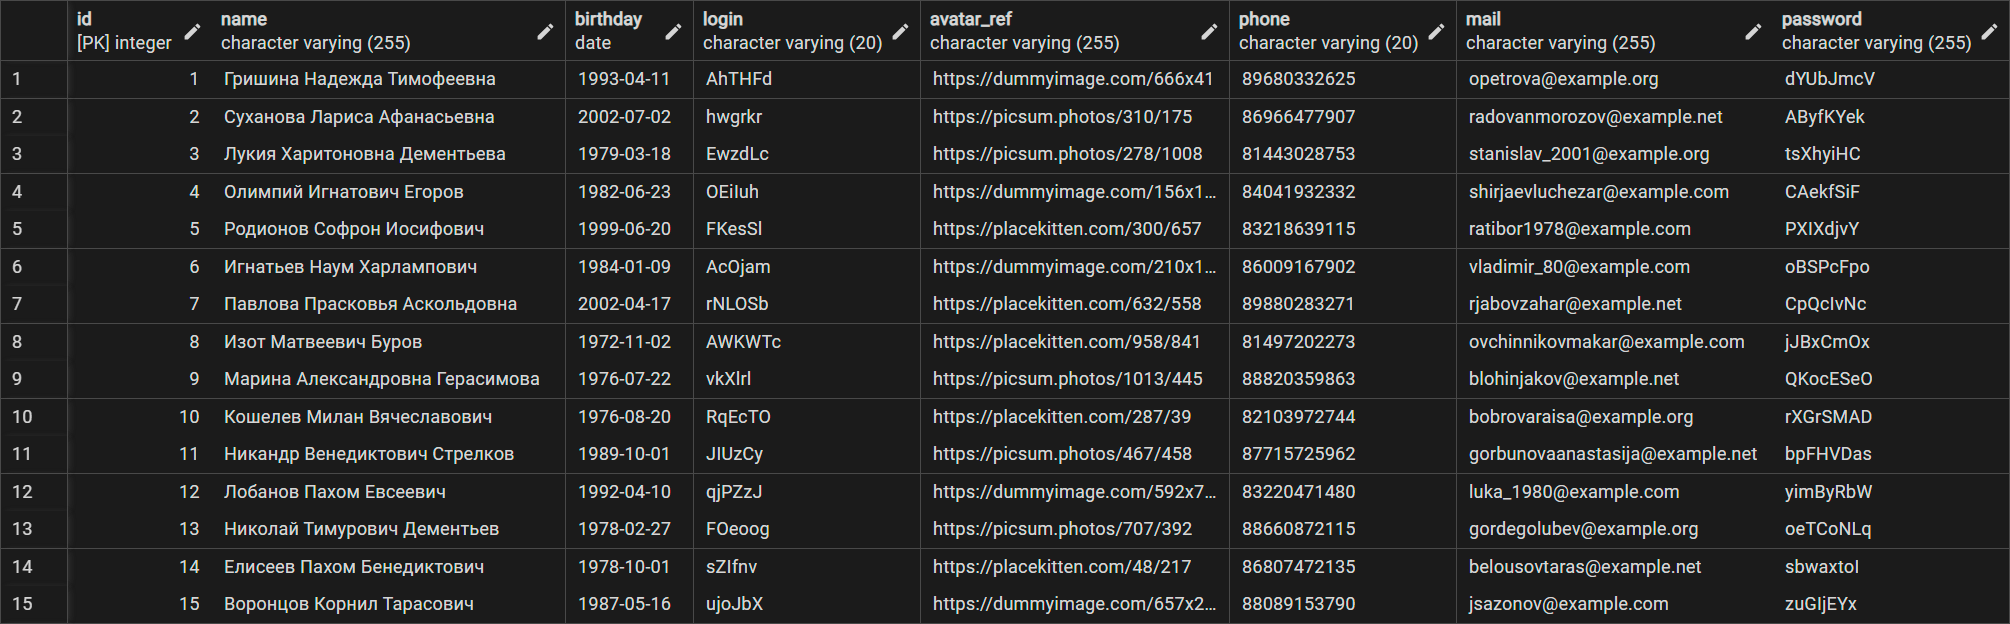
\includegraphics[scale=0.24,page=1]{Customers.png}
	$\\$
	
	
	\item Таблица Orders
	
	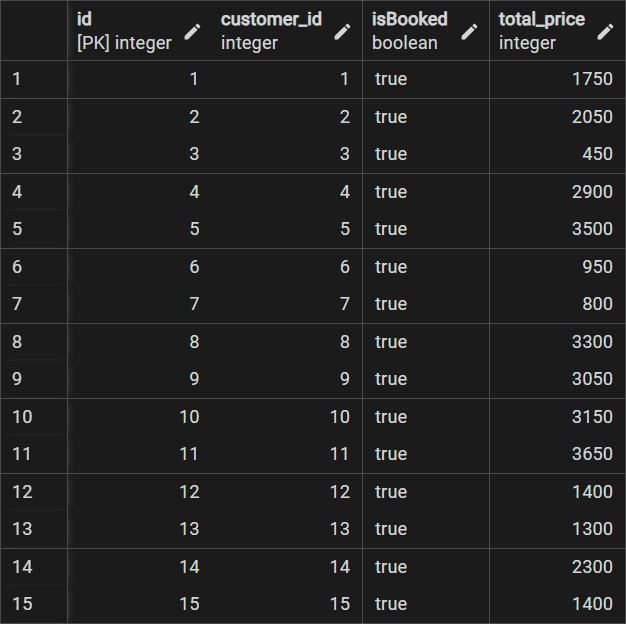
\includegraphics[scale=0.32,page=1]{Orders.png}
	$\\$
	
	
	\item Таблица Payment
	
	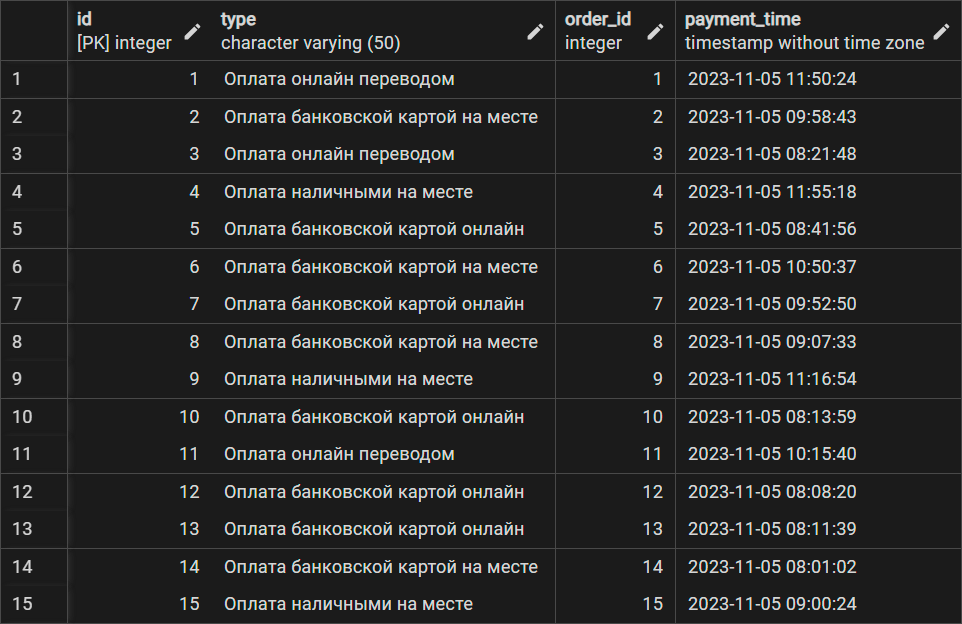
\includegraphics[scale=0.3,page=1]{Payment.png}
	$\\$
	
	
	\item Таблица Tickets
	
	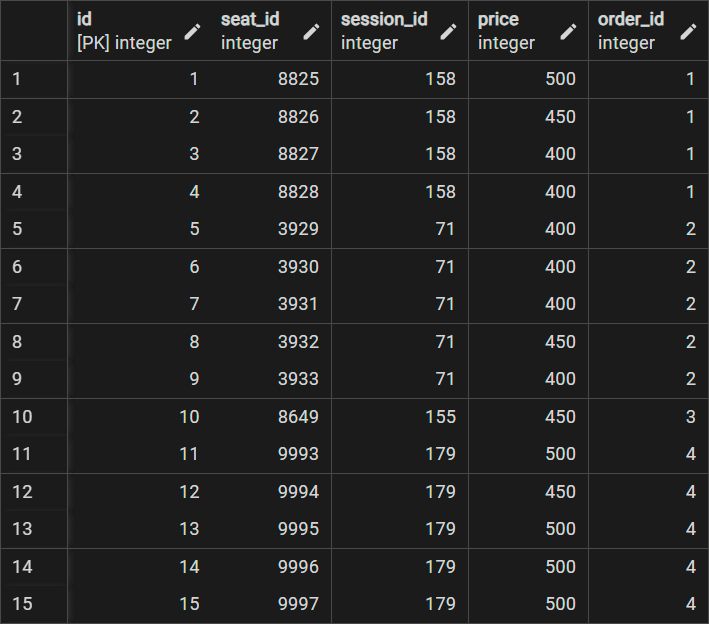
\includegraphics[scale=0.3,page=1]{Tickets.png}
	$\\$
	
	
	\item Таблица Cinemas\_positions
	
	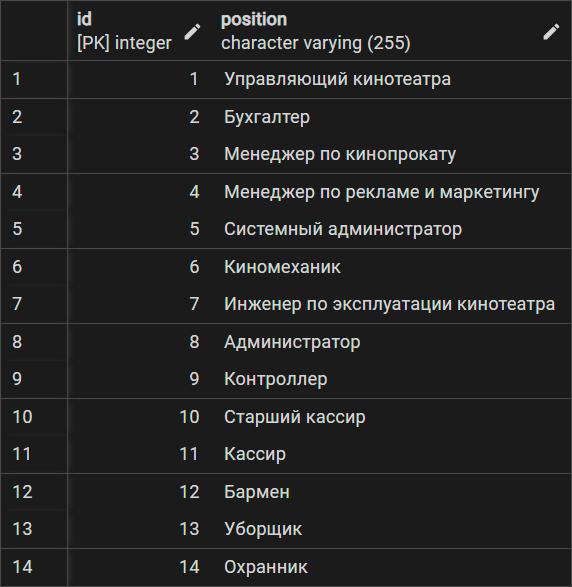
\includegraphics[scale=0.3,page=1]{Cinemas_positions.png}
	$\\$
	
	
	\item Таблица Staff
	
	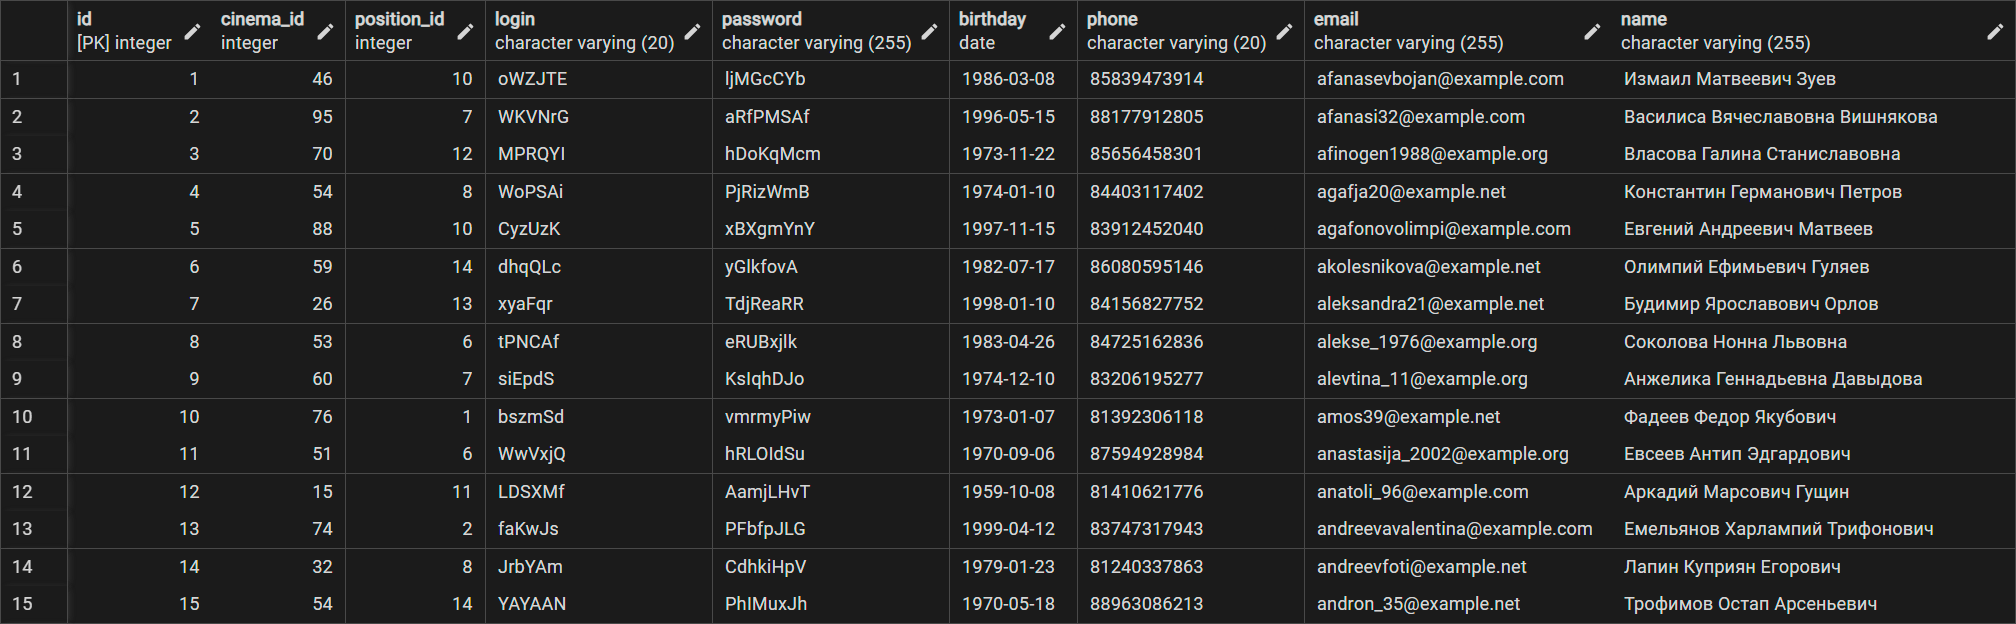
\includegraphics[scale=0.24,page=1]{Staff.png}
	
	
		
	\end{itemize}
	
	\newpage
	
	\section{Выполнение запросов}
	
	
\end{document}